% Options for packages loaded elsewhere
\PassOptionsToPackage{unicode}{hyperref}
\PassOptionsToPackage{hyphens}{url}
%
\documentclass[
]{article}
\usepackage{amsmath,amssymb}
\usepackage{iftex}
\ifPDFTeX
  \usepackage[T1]{fontenc}
  \usepackage[utf8]{inputenc}
  \usepackage{textcomp} % provide euro and other symbols
\else % if luatex or xetex
  \usepackage{unicode-math} % this also loads fontspec
  \defaultfontfeatures{Scale=MatchLowercase}
  \defaultfontfeatures[\rmfamily]{Ligatures=TeX,Scale=1}
\fi
\usepackage{lmodern}
\ifPDFTeX\else
  % xetex/luatex font selection
\fi
% Use upquote if available, for straight quotes in verbatim environments
\IfFileExists{upquote.sty}{\usepackage{upquote}}{}
\IfFileExists{microtype.sty}{% use microtype if available
  \usepackage[]{microtype}
  \UseMicrotypeSet[protrusion]{basicmath} % disable protrusion for tt fonts
}{}
\makeatletter
\@ifundefined{KOMAClassName}{% if non-KOMA class
  \IfFileExists{parskip.sty}{%
    \usepackage{parskip}
  }{% else
    \setlength{\parindent}{0pt}
    \setlength{\parskip}{6pt plus 2pt minus 1pt}}
}{% if KOMA class
  \KOMAoptions{parskip=half}}
\makeatother
\usepackage{xcolor}
\usepackage[margin=1in]{geometry}
\usepackage{color}
\usepackage{fancyvrb}
\newcommand{\VerbBar}{|}
\newcommand{\VERB}{\Verb[commandchars=\\\{\}]}
\DefineVerbatimEnvironment{Highlighting}{Verbatim}{commandchars=\\\{\}}
% Add ',fontsize=\small' for more characters per line
\usepackage{framed}
\definecolor{shadecolor}{RGB}{248,248,248}
\newenvironment{Shaded}{\begin{snugshade}}{\end{snugshade}}
\newcommand{\AlertTok}[1]{\textcolor[rgb]{0.94,0.16,0.16}{#1}}
\newcommand{\AnnotationTok}[1]{\textcolor[rgb]{0.56,0.35,0.01}{\textbf{\textit{#1}}}}
\newcommand{\AttributeTok}[1]{\textcolor[rgb]{0.13,0.29,0.53}{#1}}
\newcommand{\BaseNTok}[1]{\textcolor[rgb]{0.00,0.00,0.81}{#1}}
\newcommand{\BuiltInTok}[1]{#1}
\newcommand{\CharTok}[1]{\textcolor[rgb]{0.31,0.60,0.02}{#1}}
\newcommand{\CommentTok}[1]{\textcolor[rgb]{0.56,0.35,0.01}{\textit{#1}}}
\newcommand{\CommentVarTok}[1]{\textcolor[rgb]{0.56,0.35,0.01}{\textbf{\textit{#1}}}}
\newcommand{\ConstantTok}[1]{\textcolor[rgb]{0.56,0.35,0.01}{#1}}
\newcommand{\ControlFlowTok}[1]{\textcolor[rgb]{0.13,0.29,0.53}{\textbf{#1}}}
\newcommand{\DataTypeTok}[1]{\textcolor[rgb]{0.13,0.29,0.53}{#1}}
\newcommand{\DecValTok}[1]{\textcolor[rgb]{0.00,0.00,0.81}{#1}}
\newcommand{\DocumentationTok}[1]{\textcolor[rgb]{0.56,0.35,0.01}{\textbf{\textit{#1}}}}
\newcommand{\ErrorTok}[1]{\textcolor[rgb]{0.64,0.00,0.00}{\textbf{#1}}}
\newcommand{\ExtensionTok}[1]{#1}
\newcommand{\FloatTok}[1]{\textcolor[rgb]{0.00,0.00,0.81}{#1}}
\newcommand{\FunctionTok}[1]{\textcolor[rgb]{0.13,0.29,0.53}{\textbf{#1}}}
\newcommand{\ImportTok}[1]{#1}
\newcommand{\InformationTok}[1]{\textcolor[rgb]{0.56,0.35,0.01}{\textbf{\textit{#1}}}}
\newcommand{\KeywordTok}[1]{\textcolor[rgb]{0.13,0.29,0.53}{\textbf{#1}}}
\newcommand{\NormalTok}[1]{#1}
\newcommand{\OperatorTok}[1]{\textcolor[rgb]{0.81,0.36,0.00}{\textbf{#1}}}
\newcommand{\OtherTok}[1]{\textcolor[rgb]{0.56,0.35,0.01}{#1}}
\newcommand{\PreprocessorTok}[1]{\textcolor[rgb]{0.56,0.35,0.01}{\textit{#1}}}
\newcommand{\RegionMarkerTok}[1]{#1}
\newcommand{\SpecialCharTok}[1]{\textcolor[rgb]{0.81,0.36,0.00}{\textbf{#1}}}
\newcommand{\SpecialStringTok}[1]{\textcolor[rgb]{0.31,0.60,0.02}{#1}}
\newcommand{\StringTok}[1]{\textcolor[rgb]{0.31,0.60,0.02}{#1}}
\newcommand{\VariableTok}[1]{\textcolor[rgb]{0.00,0.00,0.00}{#1}}
\newcommand{\VerbatimStringTok}[1]{\textcolor[rgb]{0.31,0.60,0.02}{#1}}
\newcommand{\WarningTok}[1]{\textcolor[rgb]{0.56,0.35,0.01}{\textbf{\textit{#1}}}}
\usepackage{longtable,booktabs,array}
\usepackage{calc} % for calculating minipage widths
% Correct order of tables after \paragraph or \subparagraph
\usepackage{etoolbox}
\makeatletter
\patchcmd\longtable{\par}{\if@noskipsec\mbox{}\fi\par}{}{}
\makeatother
% Allow footnotes in longtable head/foot
\IfFileExists{footnotehyper.sty}{\usepackage{footnotehyper}}{\usepackage{footnote}}
\makesavenoteenv{longtable}
\usepackage{graphicx}
\makeatletter
\def\maxwidth{\ifdim\Gin@nat@width>\linewidth\linewidth\else\Gin@nat@width\fi}
\def\maxheight{\ifdim\Gin@nat@height>\textheight\textheight\else\Gin@nat@height\fi}
\makeatother
% Scale images if necessary, so that they will not overflow the page
% margins by default, and it is still possible to overwrite the defaults
% using explicit options in \includegraphics[width, height, ...]{}
\setkeys{Gin}{width=\maxwidth,height=\maxheight,keepaspectratio}
% Set default figure placement to htbp
\makeatletter
\def\fps@figure{htbp}
\makeatother
\setlength{\emergencystretch}{3em} % prevent overfull lines
\providecommand{\tightlist}{%
  \setlength{\itemsep}{0pt}\setlength{\parskip}{0pt}}
\setcounter{secnumdepth}{-\maxdimen} % remove section numbering
\ifLuaTeX
  \usepackage{selnolig}  % disable illegal ligatures
\fi
\usepackage{bookmark}
\IfFileExists{xurl.sty}{\usepackage{xurl}}{} % add URL line breaks if available
\urlstyle{same}
\hypersetup{
  pdftitle={Visualization},
  pdfauthor={Polly Wu (rw3031)},
  hidelinks,
  pdfcreator={LaTeX via pandoc}}

\title{Visualization}
\author{Polly Wu (rw3031)}
\date{2024-11-07}

\begin{document}
\maketitle

\begin{Shaded}
\begin{Highlighting}[]
\FunctionTok{library}\NormalTok{(tidyverse)}
\end{Highlighting}
\end{Shaded}

\begin{verbatim}
## -- Attaching core tidyverse packages ------------------------ tidyverse 2.0.0 --
## v dplyr     1.1.4     v readr     2.1.5
## v forcats   1.0.0     v stringr   1.5.1
## v ggplot2   3.5.1     v tibble    3.2.1
## v lubridate 1.9.3     v tidyr     1.3.1
## v purrr     1.0.2     
## -- Conflicts ------------------------------------------ tidyverse_conflicts() --
## x dplyr::filter() masks stats::filter()
## x dplyr::lag()    masks stats::lag()
## i Use the conflicted package (<http://conflicted.r-lib.org/>) to force all conflicts to become errors
\end{verbatim}

\begin{Shaded}
\begin{Highlighting}[]
\FunctionTok{library}\NormalTok{(readxl)}
\FunctionTok{library}\NormalTok{(ggplot2)}
\FunctionTok{library}\NormalTok{(rworldmap)}
\end{Highlighting}
\end{Shaded}

\begin{verbatim}
## Loading required package: sp
## ### Welcome to rworldmap ###
## For a short introduction type :   vignette('rworldmap')
\end{verbatim}

\begin{Shaded}
\begin{Highlighting}[]
\NormalTok{data\_extract }\OtherTok{=} 
  \FunctionTok{read\_excel}\NormalTok{(}\StringTok{"./Data Extraction Sheet.xlsx"}\NormalTok{)}\SpecialCharTok{|\textgreater{}}
\NormalTok{  janitor}\SpecialCharTok{::}\FunctionTok{clean\_names}\NormalTok{()}
\end{Highlighting}
\end{Shaded}

\section{the plot for year of
publication}\label{the-plot-for-year-of-publication}

\begin{Shaded}
\begin{Highlighting}[]
\NormalTok{year\_plot }\OtherTok{=}
\NormalTok{data\_extract}\SpecialCharTok{|\textgreater{}}
  \FunctionTok{ggplot}\NormalTok{(}\FunctionTok{aes}\NormalTok{(}\AttributeTok{x=}\NormalTok{year))}\SpecialCharTok{+}\FunctionTok{geom\_histogram}\NormalTok{( }\AttributeTok{fill =} \StringTok{"\#08519c"}\NormalTok{)}\SpecialCharTok{+}
  \FunctionTok{theme\_classic}\NormalTok{()}\SpecialCharTok{+}
  \FunctionTok{labs}\NormalTok{(}\AttributeTok{x =} \StringTok{"Year of Publication"}\NormalTok{,}
       \AttributeTok{title =} \StringTok{"Distribution of Year of Publication"}\NormalTok{)}

\NormalTok{year\_plot}
\end{Highlighting}
\end{Shaded}

\begin{verbatim}
## `stat_bin()` using `bins = 30`. Pick better value with `binwidth`.
\end{verbatim}

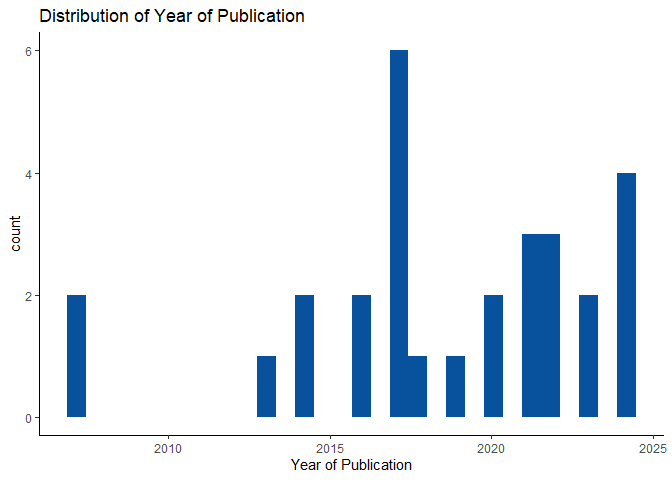
\includegraphics{visualization-for-result_files/figure-latex/unnamed-chunk-3-1.pdf}

\begin{Shaded}
\begin{Highlighting}[]
\FunctionTok{ggsave}\NormalTok{(}\StringTok{"year\_visualization.png"}\NormalTok{, }\AttributeTok{plot =}\NormalTok{ year\_plot)}
\end{Highlighting}
\end{Shaded}

\begin{verbatim}
## Saving 6.5 x 4.5 in image
## `stat_bin()` using `bins = 30`. Pick better value with `binwidth`.
\end{verbatim}

\section{the plot for geographic region of
publication}\label{the-plot-for-geographic-region-of-publication}

\begin{Shaded}
\begin{Highlighting}[]
\NormalTok{country\_count }\OtherTok{=}
\NormalTok{data\_extract}\SpecialCharTok{|\textgreater{}}
  \FunctionTok{select}\NormalTok{(country\_region)}\SpecialCharTok{|\textgreater{}}
  \FunctionTok{mutate}\NormalTok{(}\AttributeTok{country\_region =} \FunctionTok{gsub}\NormalTok{(}\StringTok{"10 clinics across "}\NormalTok{, }\StringTok{""}\NormalTok{, country\_region)) }\SpecialCharTok{|\textgreater{}}
  \FunctionTok{separate\_rows}\NormalTok{(country\_region, }\AttributeTok{sep =} \StringTok{", "}\NormalTok{) }\SpecialCharTok{|\textgreater{}}
  \FunctionTok{mutate}\NormalTok{(}\AttributeTok{country\_region =} \FunctionTok{trimws}\NormalTok{(country\_region))}\SpecialCharTok{|\textgreater{}}
  \FunctionTok{mutate}\NormalTok{(}\AttributeTok{country\_region =} \FunctionTok{str\_replace}\NormalTok{(country\_region, }\StringTok{"Hong Kong/China"}\NormalTok{, }\StringTok{"Hong Kong"}\NormalTok{),}
         \AttributeTok{country\_region =} \FunctionTok{str\_replace}\NormalTok{(country\_region, }\StringTok{"and Sweden"}\NormalTok{, }\StringTok{"Sweden"}\NormalTok{),}
         \AttributeTok{country\_region =} \FunctionTok{str\_replace}\NormalTok{(country\_region, }\StringTok{"US"}\NormalTok{, }\StringTok{"United States"}\NormalTok{)}
\NormalTok{         )}\SpecialCharTok{|\textgreater{}}
  \FunctionTok{group\_by}\NormalTok{(country\_region)}\SpecialCharTok{|\textgreater{}}
  \FunctionTok{summarise}\NormalTok{(}\AttributeTok{count=}\FunctionTok{n}\NormalTok{())}

\NormalTok{country\_count}\SpecialCharTok{|\textgreater{}}
\NormalTok{  knitr}\SpecialCharTok{::}\FunctionTok{kable}\NormalTok{()}
\end{Highlighting}
\end{Shaded}

\begin{longtable}[]{@{}lr@{}}
\toprule\noalign{}
country\_region & count \\
\midrule\noalign{}
\endhead
\bottomrule\noalign{}
\endlastfoot
Belgium & 1 \\
China & 1 \\
Estonia & 1 \\
Finland & 1 \\
France & 4 \\
Greece & 1 \\
Hong Kong & 1 \\
Japan & 1 \\
Korea & 1 \\
Netherlands & 4 \\
Norway & 1 \\
Portugal & 1 \\
Scotland & 1 \\
Spain & 2 \\
Sweden & 1 \\
Taiwan & 1 \\
United Kingdom & 1 \\
United States & 11 \\
\end{longtable}

\begin{Shaded}
\begin{Highlighting}[]
\NormalTok{world\_map }\OtherTok{\textless{}{-}} \FunctionTok{joinCountryData2Map}\NormalTok{(country\_count, }\AttributeTok{joinCode =} \StringTok{"NAME"}\NormalTok{, }\AttributeTok{nameJoinColumn =} \StringTok{"country\_region"}\NormalTok{)}
\end{Highlighting}
\end{Shaded}

\begin{verbatim}
## 17 codes from your data successfully matched countries in the map
## 1 codes from your data failed to match with a country code in the map
## 226 codes from the map weren't represented in your data
\end{verbatim}

\begin{Shaded}
\begin{Highlighting}[]
\NormalTok{blue\_palette }\OtherTok{\textless{}{-}} \FunctionTok{rev}\NormalTok{(}\FunctionTok{c}\NormalTok{(}\StringTok{"\#08306b"}\NormalTok{, }\StringTok{"\#08519c"}\NormalTok{, }\StringTok{"\#2171b5"}\NormalTok{, }\StringTok{"\#4292c6"}\NormalTok{, }\StringTok{"\#6baed6"}\NormalTok{, }\StringTok{"\#9ecae1"}\NormalTok{, }\StringTok{"\#c6dbef"}\NormalTok{, }\StringTok{"\#deebf7"}\NormalTok{))}

\FunctionTok{png}\NormalTok{(}\StringTok{"map\_visualization.png"}\NormalTok{, }\AttributeTok{width =} \DecValTok{800}\NormalTok{, }\AttributeTok{height =} \DecValTok{600}\NormalTok{)}

\FunctionTok{mapCountryData}\NormalTok{(world\_map, }\AttributeTok{nameColumnToPlot =} \StringTok{"count"}\NormalTok{, }\AttributeTok{catMethod =} \StringTok{"fixedWidth"}\NormalTok{, }\AttributeTok{colourPalette =}\NormalTok{ blue\_palette, }\AttributeTok{mapTitle =} \StringTok{"Geographic Distribution regarding Publications"}\NormalTok{)}
\end{Highlighting}
\end{Shaded}

\begin{verbatim}
## Warning in rwmGetColours(colourPalette, numColours): 8 colours specified and 7
## required, using interpolation to calculate colours
\end{verbatim}

\begin{Shaded}
\begin{Highlighting}[]
\FunctionTok{dev.off}\NormalTok{()}
\end{Highlighting}
\end{Shaded}

\begin{verbatim}
## pdf 
##   2
\end{verbatim}

\section{type of interventions}\label{type-of-interventions}

\begin{Shaded}
\begin{Highlighting}[]
\NormalTok{data\_extract}\SpecialCharTok{|\textgreater{}}
  \FunctionTok{group\_by}\NormalTok{(intervention\_type)}\SpecialCharTok{|\textgreater{}}
  \FunctionTok{summarise}\NormalTok{(}\AttributeTok{count =} \FunctionTok{n}\NormalTok{())}\SpecialCharTok{|\textgreater{}}
  \FunctionTok{arrange}\NormalTok{(}\FunctionTok{desc}\NormalTok{(count))}
\end{Highlighting}
\end{Shaded}

\begin{verbatim}
## # A tibble: 6 x 2
##   intervention_type                   count
##   <chr>                               <int>
## 1 mobile application                      8
## 2 telemedicine                            8
## 3 website/online platform                 8
## 4 electronic questionnaire/assessment     2
## 5 wearable device                         2
## 6 virtual reality                         1
\end{verbatim}

\begin{Shaded}
\begin{Highlighting}[]
\NormalTok{data\_extract}\SpecialCharTok{|\textgreater{}}
  \FunctionTok{select}\NormalTok{(id,intervention\_type)}\SpecialCharTok{|\textgreater{}}
  \FunctionTok{arrange}\NormalTok{(}\FunctionTok{desc}\NormalTok{(intervention\_type))}
\end{Highlighting}
\end{Shaded}

\begin{verbatim}
## # A tibble: 29 x 2
##       id intervention_type      
##    <dbl> <chr>                  
##  1     5 website/online platform
##  2     6 website/online platform
##  3    11 website/online platform
##  4    16 website/online platform
##  5    17 website/online platform
##  6    18 website/online platform
##  7    22 website/online platform
##  8    24 website/online platform
##  9    20 wearable device        
## 10    28 wearable device        
## # i 19 more rows
\end{verbatim}

\subsection{settings}\label{settings}

\begin{Shaded}
\begin{Highlighting}[]
\NormalTok{data\_extract}\SpecialCharTok{|\textgreater{}}
  \FunctionTok{group\_by}\NormalTok{(setting)}\SpecialCharTok{|\textgreater{}}
  \FunctionTok{summarise}\NormalTok{(}\AttributeTok{count =} \FunctionTok{n}\NormalTok{())}\SpecialCharTok{|\textgreater{}}
  \FunctionTok{arrange}\NormalTok{(}\FunctionTok{desc}\NormalTok{(count))}
\end{Highlighting}
\end{Shaded}

\begin{verbatim}
## # A tibble: 3 x 2
##   setting        count
##   <chr>          <int>
## 1 home-based        23
## 2 clinical based     4
## 3 both               2
\end{verbatim}

\begin{Shaded}
\begin{Highlighting}[]
\NormalTok{data\_extract}\SpecialCharTok{|\textgreater{}}
  \FunctionTok{filter}\NormalTok{(setting }\SpecialCharTok{==} \StringTok{"home{-}based"}\NormalTok{)}
\end{Highlighting}
\end{Shaded}

\begin{verbatim}
## # A tibble: 23 x 34
##       id title   year objective study_design intervention who_is_delivering_th~1
##    <dbl> <chr>  <dbl> <chr>     <chr>        <chr>        <chr>                 
##  1     1 Telem~  2023 We inves~ "a parallel~ 12-week int~ trainer               
##  2     2 Testi~  2024 Test the~ "Structured~ A Lalaby Ap~ Research team         
##  3     3 Mobil~  2019 determin~ "prospectiv~ A comprehen~ Physician             
##  4     4 Co-cr~  2016 To devel~ "User-cente~ A telehealt~ physiotherapists, sur~
##  5     5 Why D~  2014 Explore ~ "Qualitativ~ Web-based Q~ Physician             
##  6     6 Evalu~  2022 Evaluate~ "Mixed-meth~ Digital pla~ oncologists, nurses, ~
##  7     8 Pilot~  2020 Assess t~ "Pilot stud~ Telehealth ~ Physical and occupati~
##  8     9 Exper~  2017 Tests ne~ "survey, qu~ Patients co~ Lung cancer nurse spe~
##  9    12 Teleh~  2024 To evalu~ "Multisite ~ Early palli~ Physician             
## 10    14 Impro~  2017 To evalu~ "Retrospect~ self-report~ Physician             
## # i 13 more rows
## # i abbreviated name: 1: who_is_delivering_the_intervention
## # i 27 more variables: setting <chr>, length_of_interventions <chr>,
## #   frequency_of_interventions <chr>,
## #   theory_or_non_theory_based_is_it_guided_by_a_specific_framework <chr>,
## #   country_region <chr>, patient_demographics <chr>, age_range <chr>,
## #   stage_of_cancer <chr>, stage_2 <chr>, ...
\end{verbatim}

\subsection{stage}\label{stage}

\begin{Shaded}
\begin{Highlighting}[]
\NormalTok{data\_extract}\SpecialCharTok{|\textgreater{}}
  \FunctionTok{select}\NormalTok{(id,stage\_2)}\SpecialCharTok{|\textgreater{}}
  \FunctionTok{arrange}\NormalTok{(}\FunctionTok{desc}\NormalTok{(stage\_2))}
\end{Highlighting}
\end{Shaded}

\begin{verbatim}
## # A tibble: 29 x 2
##       id stage_2             
##    <dbl> <chr>               
##  1     1 local and metastatic
##  2     3 local and metastatic
##  3     5 local and metastatic
##  4     6 local and metastatic
##  5     7 local and metastatic
##  6    14 local and metastatic
##  7    20 local and metastatic
##  8    21 local and metastatic
##  9    23 local and metastatic
## 10    24 local and metastatic
## # i 19 more rows
\end{verbatim}

\begin{Shaded}
\begin{Highlighting}[]
\NormalTok{data\_extract}\SpecialCharTok{|\textgreater{}}
  \FunctionTok{select}\NormalTok{(id,stage\_2)}\SpecialCharTok{|\textgreater{}}
  \FunctionTok{group\_by}\NormalTok{(stage\_2)}\SpecialCharTok{|\textgreater{}}
  \FunctionTok{summarise}\NormalTok{(}\FunctionTok{n}\NormalTok{())}
\end{Highlighting}
\end{Shaded}

\begin{verbatim}
## # A tibble: 4 x 2
##   stage_2                    `n()`
##   <chr>                      <int>
## 1 Advanced stage, metastatic     8
## 2 NA                             8
## 3 local                          1
## 4 local and metastatic          12
\end{verbatim}

\subsection{treatment type}\label{treatment-type}

\begin{Shaded}
\begin{Highlighting}[]
\NormalTok{data\_extract}\SpecialCharTok{|\textgreater{}}
  \FunctionTok{select}\NormalTok{(treatment\_2,id)}\SpecialCharTok{|\textgreater{}}
  \FunctionTok{separate\_rows}\NormalTok{(treatment\_2, }\AttributeTok{sep =} \StringTok{","}\NormalTok{)}\SpecialCharTok{|\textgreater{}}
  \FunctionTok{group\_by}\NormalTok{(treatment\_2)}\SpecialCharTok{|\textgreater{}}
  \FunctionTok{summarise}\NormalTok{(}\AttributeTok{id=}\FunctionTok{paste}\NormalTok{(}\FunctionTok{unique}\NormalTok{(id),}\AttributeTok{collapse =} \StringTok{","}\NormalTok{), }\AttributeTok{count =} \FunctionTok{n}\NormalTok{())}
\end{Highlighting}
\end{Shaded}

\begin{verbatim}
## # A tibble: 7 x 3
##   treatment_2        id                                    count
##   <chr>              <chr>                                 <int>
## 1 chemotherapy       1,2,3,5,6,7,9,10,12,14,15,21,23,24,26    15
## 2 immunotherapy      6,7,29                                    3
## 3 not specified      11,13,16,18,19,20,22                      7
## 4 palliative/hospice 27,28                                     2
## 5 radiotherapy       1,9,14,21,24,25                           6
## 6 surgery            1,4,5,8,9,14,17,21,24,25                 10
## 7 targeted therapy   7,21                                      2
\end{verbatim}

\subsection{challenge faced by patients in different treatment
regimens}\label{challenge-faced-by-patients-in-different-treatment-regimens}

\begin{Shaded}
\begin{Highlighting}[]
\NormalTok{data\_extract}\SpecialCharTok{|\textgreater{}}
  \FunctionTok{select}\NormalTok{(challenge\_recode, treatment\_2, id)}\SpecialCharTok{|\textgreater{}}
  \FunctionTok{separate\_rows}\NormalTok{(challenge\_recode, }\AttributeTok{sep =} \StringTok{","}\NormalTok{)}\SpecialCharTok{|\textgreater{}}
  \FunctionTok{group\_by}\NormalTok{(challenge\_recode)}\SpecialCharTok{|\textgreater{}}
  \FunctionTok{summarise}\NormalTok{(}\AttributeTok{count =} \FunctionTok{n}\NormalTok{(),}
            \AttributeTok{id=}\FunctionTok{paste}\NormalTok{(}\FunctionTok{unique}\NormalTok{(id),}\AttributeTok{collapse =} \StringTok{","}\NormalTok{))}\SpecialCharTok{|\textgreater{}}
  \FunctionTok{arrange}\NormalTok{(}\FunctionTok{desc}\NormalTok{(count))}
\end{Highlighting}
\end{Shaded}

\begin{verbatim}
## # A tibble: 6 x 3
##   challenge_recode                              count id                        
##   <chr>                                         <int> <chr>                     
## 1 symptom distress/side-effect management          23 1,2,3,4,6,7,8,10,11,12,14~
## 2 emotional distress/anxiety/depression            12 1,5,6,8,10,12,16,17,19,24~
## 3 accurate and in-time reporting of symptoms       10 2,6,7,13,14,21,22,23,27,28
## 4 communication with providers                      8 2,4,6,7,9,14,15,25        
## 5 adherence to rehabilitation/physical activity     7 1,3,4,8,18,24,29          
## 6 preparedness for treatment                        3 5,8,16
\end{verbatim}

\begin{Shaded}
\begin{Highlighting}[]
\NormalTok{data\_extract}\SpecialCharTok{|\textgreater{}}
  \FunctionTok{select}\NormalTok{(challenge\_recode, treatment\_2, id)}\SpecialCharTok{|\textgreater{}}
  \FunctionTok{separate\_rows}\NormalTok{(challenge\_recode, }\AttributeTok{sep =} \StringTok{","}\NormalTok{)}\SpecialCharTok{|\textgreater{}}
  \FunctionTok{separate\_rows}\NormalTok{(treatment\_2, }\AttributeTok{sep =} \StringTok{","}\NormalTok{)}\SpecialCharTok{|\textgreater{}}
  \FunctionTok{group\_by}\NormalTok{(challenge\_recode, treatment\_2)}\SpecialCharTok{|\textgreater{}}
  \FunctionTok{summarise}\NormalTok{(}\AttributeTok{count =} \FunctionTok{n}\NormalTok{(),}
            \AttributeTok{id=}\FunctionTok{paste}\NormalTok{(}\FunctionTok{unique}\NormalTok{(id),}\AttributeTok{collapse =} \StringTok{","}\NormalTok{))}\SpecialCharTok{|\textgreater{}}
  \FunctionTok{arrange}\NormalTok{(treatment\_2, }\FunctionTok{desc}\NormalTok{(count))}
\end{Highlighting}
\end{Shaded}

\begin{verbatim}
## `summarise()` has grouped output by 'challenge_recode'. You can override using
## the `.groups` argument.
\end{verbatim}

\begin{verbatim}
## # A tibble: 33 x 4
## # Groups:   challenge_recode [6]
##    challenge_recode                              treatment_2   count id         
##    <chr>                                         <chr>         <int> <chr>      
##  1 symptom distress/side-effect management       chemotherapy     13 1,2,3,6,7,~
##  2 accurate and in-time reporting of symptoms    chemotherapy      6 2,6,7,14,2~
##  3 communication with providers                  chemotherapy      6 2,6,7,9,14~
##  4 emotional distress/anxiety/depression         chemotherapy      6 1,5,6,10,1~
##  5 adherence to rehabilitation/physical activity chemotherapy      3 1,3,24     
##  6 preparedness for treatment                    chemotherapy      1 5          
##  7 accurate and in-time reporting of symptoms    immunotherapy     2 6,7        
##  8 communication with providers                  immunotherapy     2 6,7        
##  9 emotional distress/anxiety/depression         immunotherapy     2 6,29       
## 10 symptom distress/side-effect management       immunotherapy     2 6,7        
## # i 23 more rows
\end{verbatim}

\subsection{intervention design * type}\label{intervention-design-type}

\begin{Shaded}
\begin{Highlighting}[]
\NormalTok{data\_extract}\SpecialCharTok{|\textgreater{}}
  \FunctionTok{select}\NormalTok{(id,intervention\_type,commercial\_tool\_designed\_specifically\_for\_the\_study)}\SpecialCharTok{|\textgreater{}}
  \FunctionTok{group\_by}\NormalTok{(intervention\_type,commercial\_tool\_designed\_specifically\_for\_the\_study)}\SpecialCharTok{|\textgreater{}}
  \FunctionTok{summarise}\NormalTok{(}\AttributeTok{id=}\FunctionTok{paste}\NormalTok{(}\FunctionTok{unique}\NormalTok{(id),}\AttributeTok{collapse =} \StringTok{","}\NormalTok{))}\SpecialCharTok{|\textgreater{}}
  \FunctionTok{pivot\_wider}\NormalTok{(}
    \AttributeTok{values\_from =}\NormalTok{ id,}
    \AttributeTok{names\_from =}\NormalTok{ commercial\_tool\_designed\_specifically\_for\_the\_study}
\NormalTok{  )}
\end{Highlighting}
\end{Shaded}

\begin{verbatim}
## `summarise()` has grouped output by 'intervention_type'. You can override using
## the `.groups` argument.
\end{verbatim}

\begin{verbatim}
## # A tibble: 6 x 3
## # Groups:   intervention_type [6]
##   intervention_type                   `designed for the study` `commercial tool`
##   <chr>                               <chr>                    <chr>            
## 1 electronic questionnaire/assessment 7,13                     <NA>             
## 2 mobile application                  2,3,4,14,21,23,27        15               
## 3 telemedicine                        1,12,19,26               8,9,25,29        
## 4 virtual reality                     <NA>                     10               
## 5 wearable device                     28                       20               
## 6 website/online platform             6,11,16,17,18,22,24      5
\end{verbatim}

\begin{Shaded}
\begin{Highlighting}[]
\NormalTok{data\_extract}\SpecialCharTok{|\textgreater{}}
  \FunctionTok{select}\NormalTok{(id,pre\_post,intervention\_type)}\SpecialCharTok{|\textgreater{}}
  \FunctionTok{mutate}\NormalTok{(}
    \AttributeTok{Pre\_treatment =} \FunctionTok{ifelse}\NormalTok{(}\FunctionTok{str\_detect}\NormalTok{(pre\_post, }\StringTok{"Pre{-}treatment"}\NormalTok{), }\DecValTok{1}\NormalTok{, }\DecValTok{0}\NormalTok{),}
    \AttributeTok{During\_treatment =} \FunctionTok{ifelse}\NormalTok{(}\FunctionTok{str\_detect}\NormalTok{(pre\_post, }\StringTok{"During{-}treatment"}\NormalTok{), }\DecValTok{1}\NormalTok{, }\DecValTok{0}\NormalTok{),}
    \AttributeTok{Post\_treatment =} \FunctionTok{ifelse}\NormalTok{(}\FunctionTok{str\_detect}\NormalTok{(pre\_post, }\StringTok{"Post{-}treatment"}\NormalTok{), }\DecValTok{1}\NormalTok{, }\DecValTok{0}\NormalTok{)}
\NormalTok{  )}\SpecialCharTok{|\textgreater{}}
  \FunctionTok{group\_by}\NormalTok{(intervention\_type,pre\_post)}\SpecialCharTok{|\textgreater{}}
  \FunctionTok{summarise}\NormalTok{(}\AttributeTok{count=}\FunctionTok{n}\NormalTok{())}\SpecialCharTok{|\textgreater{}}
  \FunctionTok{pivot\_wider}\NormalTok{(}
    \AttributeTok{values\_from =}\NormalTok{ count,}
    \AttributeTok{names\_from =}\NormalTok{ pre\_post}
\NormalTok{  )}
\end{Highlighting}
\end{Shaded}

\begin{verbatim}
## `summarise()` has grouped output by 'intervention_type'. You can override using
## the `.groups` argument.
\end{verbatim}

\begin{verbatim}
## # A tibble: 6 x 7
## # Groups:   intervention_type [6]
##   intervention_type   `During-treatment` `Post-treatment` During-treatment,Pos~1
##   <chr>                            <int>            <int>                  <int>
## 1 electronic questio~                  2               NA                     NA
## 2 mobile application                   5                3                     NA
## 3 telemedicine                         4               NA                      2
## 4 virtual reality                      1               NA                     NA
## 5 wearable device                      2               NA                     NA
## 6 website/online pla~                  5                1                     NA
## # i abbreviated name: 1: `During-treatment,Post-treatment`
## # i 3 more variables: `Pre-treatment,During-treatment` <int>,
## #   `Pre-treatment,During-treatment,Post-treatment` <int>,
## #   `Pre-treatment` <int>
\end{verbatim}

\subsection{plot for pre-post over intervention
type}\label{plot-for-pre-post-over-intervention-type}

\begin{Shaded}
\begin{Highlighting}[]
\FunctionTok{library}\NormalTok{(viridis)}
\end{Highlighting}
\end{Shaded}

\begin{verbatim}
## Loading required package: viridisLite
\end{verbatim}

\begin{Shaded}
\begin{Highlighting}[]
\NormalTok{data\_extract }\SpecialCharTok{|\textgreater{}}
  \FunctionTok{select}\NormalTok{(id, pre\_post, intervention\_type) }\SpecialCharTok{|\textgreater{}}
  \FunctionTok{separate\_rows}\NormalTok{(pre\_post, }\AttributeTok{sep =} \StringTok{","}\NormalTok{) }\SpecialCharTok{|\textgreater{}}
  \FunctionTok{ggplot}\NormalTok{(}\FunctionTok{aes}\NormalTok{(}\AttributeTok{x =}\NormalTok{ intervention\_type, }\AttributeTok{fill =}\NormalTok{ pre\_post)) }\SpecialCharTok{+}
  \FunctionTok{geom\_bar}\NormalTok{() }\SpecialCharTok{+}
  \FunctionTok{scale\_fill\_viridis\_d}\NormalTok{() }\SpecialCharTok{+}
  \FunctionTok{theme}\NormalTok{(}
      \AttributeTok{legend.position =} \StringTok{"bottom"}\NormalTok{,}
      \AttributeTok{panel.background =} \FunctionTok{element\_rect}\NormalTok{(}\AttributeTok{fill =} \StringTok{"white"}\NormalTok{, }\AttributeTok{color =} \ConstantTok{NA}\NormalTok{),}
      \AttributeTok{plot.background =} \FunctionTok{element\_rect}\NormalTok{(}\AttributeTok{fill =} \StringTok{"white"}\NormalTok{, }\AttributeTok{color =} \ConstantTok{NA}\NormalTok{),}
      \AttributeTok{panel.grid.major =} \FunctionTok{element\_blank}\NormalTok{(),}
      \AttributeTok{panel.grid.minor =} \FunctionTok{element\_blank}\NormalTok{()}
\NormalTok{    )}
\end{Highlighting}
\end{Shaded}

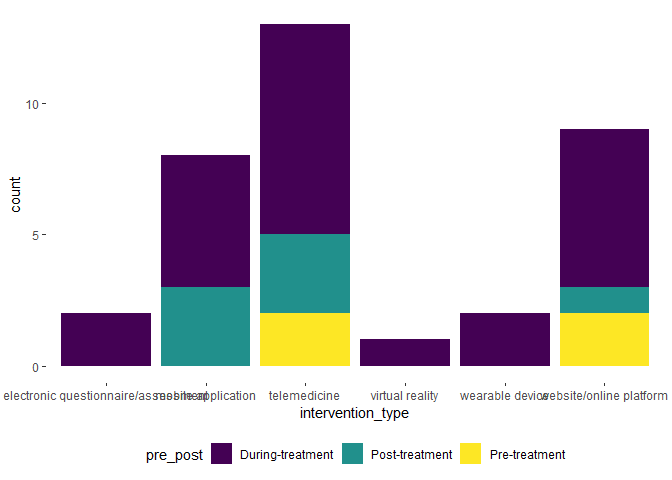
\includegraphics{visualization-for-result_files/figure-latex/unnamed-chunk-14-1.pdf}

\subsection{plot for theme over intervention
type}\label{plot-for-theme-over-intervention-type}

\begin{Shaded}
\begin{Highlighting}[]
\NormalTok{theme\_intervention }\OtherTok{=}
\NormalTok{  data\_extract }\SpecialCharTok{|\textgreater{}}
    \FunctionTok{select}\NormalTok{(theme, intervention\_type) }\SpecialCharTok{|\textgreater{}}
    \FunctionTok{separate\_rows}\NormalTok{(theme, }\AttributeTok{sep =} \StringTok{","}\NormalTok{) }\SpecialCharTok{|\textgreater{}}
    \FunctionTok{ggplot}\NormalTok{(}\FunctionTok{aes}\NormalTok{(}\AttributeTok{x =}\NormalTok{ intervention\_type, }\AttributeTok{fill =}\NormalTok{ theme)) }\SpecialCharTok{+}
    \FunctionTok{geom\_bar}\NormalTok{() }\SpecialCharTok{+}
    \FunctionTok{scale\_fill\_viridis\_d}\NormalTok{() }\SpecialCharTok{+}
    \FunctionTok{theme}\NormalTok{(}
      \AttributeTok{legend.position =} \StringTok{"bottom"}\NormalTok{,}
      \AttributeTok{panel.background =} \FunctionTok{element\_rect}\NormalTok{(}\AttributeTok{fill =} \StringTok{"white"}\NormalTok{, }\AttributeTok{color =} \ConstantTok{NA}\NormalTok{),}
      \AttributeTok{plot.background =} \FunctionTok{element\_rect}\NormalTok{(}\AttributeTok{fill =} \StringTok{"white"}\NormalTok{, }\AttributeTok{color =} \ConstantTok{NA}\NormalTok{),}
      \AttributeTok{panel.grid.major =} \FunctionTok{element\_blank}\NormalTok{(),}
      \AttributeTok{panel.grid.minor =} \FunctionTok{element\_blank}\NormalTok{()}
\NormalTok{    )}

\NormalTok{theme\_intervention}
\end{Highlighting}
\end{Shaded}

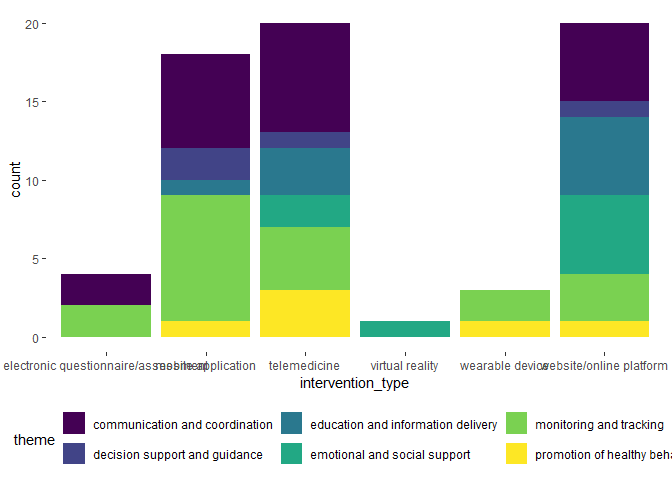
\includegraphics{visualization-for-result_files/figure-latex/unnamed-chunk-15-1.pdf}

\section{intervention type over
pre\_post}\label{intervention-type-over-pre_post}

\begin{Shaded}
\begin{Highlighting}[]
\NormalTok{data\_extract}\SpecialCharTok{|\textgreater{}}
  \FunctionTok{select}\NormalTok{(id,pre\_post,intervention\_type)}\SpecialCharTok{|\textgreater{}}
  \FunctionTok{separate\_rows}\NormalTok{(pre\_post, }\AttributeTok{sep =} \StringTok{","}\NormalTok{)}\SpecialCharTok{|\textgreater{}}
  \FunctionTok{group\_by}\NormalTok{(intervention\_type,pre\_post)}\SpecialCharTok{|\textgreater{}}
  \FunctionTok{summarise}\NormalTok{(}\AttributeTok{count =} \FunctionTok{n}\NormalTok{())}\SpecialCharTok{|\textgreater{}}
  \FunctionTok{pivot\_wider}\NormalTok{(}
    \AttributeTok{names\_from =}\NormalTok{ pre\_post,}
    \AttributeTok{values\_from =}\NormalTok{ count}
\NormalTok{  )}\SpecialCharTok{|\textgreater{}}
\NormalTok{  knitr}\SpecialCharTok{::}\FunctionTok{kable}\NormalTok{()}
\end{Highlighting}
\end{Shaded}

\begin{verbatim}
## `summarise()` has grouped output by 'intervention_type'. You can override using
## the `.groups` argument.
\end{verbatim}

\begin{longtable}[]{@{}
  >{\raggedright\arraybackslash}p{(\columnwidth - 6\tabcolsep) * \real{0.4390}}
  >{\raggedleft\arraybackslash}p{(\columnwidth - 6\tabcolsep) * \real{0.2073}}
  >{\raggedleft\arraybackslash}p{(\columnwidth - 6\tabcolsep) * \real{0.1829}}
  >{\raggedleft\arraybackslash}p{(\columnwidth - 6\tabcolsep) * \real{0.1707}}@{}}
\toprule\noalign{}
\begin{minipage}[b]{\linewidth}\raggedright
intervention\_type
\end{minipage} & \begin{minipage}[b]{\linewidth}\raggedleft
During-treatment
\end{minipage} & \begin{minipage}[b]{\linewidth}\raggedleft
Post-treatment
\end{minipage} & \begin{minipage}[b]{\linewidth}\raggedleft
Pre-treatment
\end{minipage} \\
\midrule\noalign{}
\endhead
\bottomrule\noalign{}
\endlastfoot
electronic questionnaire/assessment & 2 & NA & NA \\
mobile application & 5 & 3 & NA \\
telemedicine & 8 & 3 & 2 \\
virtual reality & 1 & NA & NA \\
wearable device & 2 & NA & NA \\
website/online platform & 6 & 1 & 2 \\
\end{longtable}

\section{intervention type over
theme}\label{intervention-type-over-theme}

\begin{Shaded}
\begin{Highlighting}[]
\NormalTok{data\_extract}\SpecialCharTok{|\textgreater{}}
  \FunctionTok{select}\NormalTok{(theme,intervention\_type)}\SpecialCharTok{|\textgreater{}}
  \FunctionTok{separate\_rows}\NormalTok{(theme, }\AttributeTok{sep =} \StringTok{","}\NormalTok{)}\SpecialCharTok{|\textgreater{}}
  \FunctionTok{group\_by}\NormalTok{(intervention\_type,theme)}\SpecialCharTok{|\textgreater{}}
  \FunctionTok{summarise}\NormalTok{(}\AttributeTok{count =} \FunctionTok{n}\NormalTok{())}\SpecialCharTok{|\textgreater{}}
  \FunctionTok{pivot\_wider}\NormalTok{(}
    \AttributeTok{names\_from =}\NormalTok{ theme,}
    \AttributeTok{values\_from =}\NormalTok{ count}
\NormalTok{  )}\SpecialCharTok{|\textgreater{}}
\NormalTok{  knitr}\SpecialCharTok{::}\FunctionTok{kable}\NormalTok{()}
\end{Highlighting}
\end{Shaded}

\begin{verbatim}
## `summarise()` has grouped output by 'intervention_type'. You can override using
## the `.groups` argument.
\end{verbatim}

\begin{longtable}[]{@{}
  >{\raggedright\arraybackslash}p{(\columnwidth - 12\tabcolsep) * \real{0.1674}}
  >{\raggedleft\arraybackslash}p{(\columnwidth - 12\tabcolsep) * \real{0.1442}}
  >{\raggedleft\arraybackslash}p{(\columnwidth - 12\tabcolsep) * \real{0.1116}}
  >{\raggedleft\arraybackslash}p{(\columnwidth - 12\tabcolsep) * \real{0.1395}}
  >{\raggedleft\arraybackslash}p{(\columnwidth - 12\tabcolsep) * \real{0.1628}}
  >{\raggedleft\arraybackslash}p{(\columnwidth - 12\tabcolsep) * \real{0.1395}}
  >{\raggedleft\arraybackslash}p{(\columnwidth - 12\tabcolsep) * \real{0.1349}}@{}}
\toprule\noalign{}
\begin{minipage}[b]{\linewidth}\raggedright
intervention\_type
\end{minipage} & \begin{minipage}[b]{\linewidth}\raggedleft
communication and coordination
\end{minipage} & \begin{minipage}[b]{\linewidth}\raggedleft
monitoring and tracking
\end{minipage} & \begin{minipage}[b]{\linewidth}\raggedleft
decision support and guidance
\end{minipage} & \begin{minipage}[b]{\linewidth}\raggedleft
education and information delivery
\end{minipage} & \begin{minipage}[b]{\linewidth}\raggedleft
promotion of healthy behavior
\end{minipage} & \begin{minipage}[b]{\linewidth}\raggedleft
emotional and social support
\end{minipage} \\
\midrule\noalign{}
\endhead
\bottomrule\noalign{}
\endlastfoot
electronic questionnaire/assessment & 2 & 2 & NA & NA & NA & NA \\
mobile application & 6 & 8 & 2 & 1 & 1 & NA \\
telemedicine & 6 & 4 & 1 & 3 & 3 & 1 \\
virtual reality & NA & NA & NA & NA & NA & 1 \\
wearable device & NA & 2 & NA & NA & 1 & NA \\
website/online platform & 4 & 3 & 1 & 5 & 1 & 5 \\
\end{longtable}

\begin{Shaded}
\begin{Highlighting}[]
\NormalTok{data\_extract}\SpecialCharTok{|\textgreater{}}
  \FunctionTok{select}\NormalTok{(theme,intervention\_type, pre\_post)}\SpecialCharTok{|\textgreater{}}
  \FunctionTok{separate\_rows}\NormalTok{(theme, }\AttributeTok{sep =} \StringTok{","}\NormalTok{)}\SpecialCharTok{|\textgreater{}}
  \FunctionTok{group\_by}\NormalTok{(intervention\_type,theme,pre\_post)}\SpecialCharTok{|\textgreater{}}
  \FunctionTok{summarise}\NormalTok{(}\AttributeTok{count =} \FunctionTok{n}\NormalTok{())}\SpecialCharTok{|\textgreater{}}
  \FunctionTok{pivot\_wider}\NormalTok{(}
    \AttributeTok{names\_from =}\NormalTok{ pre\_post,}
    \AttributeTok{values\_from =}\NormalTok{ count}
\NormalTok{  )}\SpecialCharTok{|\textgreater{}}
\NormalTok{  knitr}\SpecialCharTok{::}\FunctionTok{kable}\NormalTok{()}
\end{Highlighting}
\end{Shaded}

\begin{verbatim}
## `summarise()` has grouped output by 'intervention_type', 'theme'. You can
## override using the `.groups` argument.
\end{verbatim}

\begin{longtable}[]{@{}
  >{\raggedright\arraybackslash}p{(\columnwidth - 14\tabcolsep) * \real{0.1593}}
  >{\raggedright\arraybackslash}p{(\columnwidth - 14\tabcolsep) * \real{0.1549}}
  >{\raggedleft\arraybackslash}p{(\columnwidth - 14\tabcolsep) * \real{0.0752}}
  >{\raggedleft\arraybackslash}p{(\columnwidth - 14\tabcolsep) * \real{0.0664}}
  >{\raggedleft\arraybackslash}p{(\columnwidth - 14\tabcolsep) * \real{0.1416}}
  >{\raggedleft\arraybackslash}p{(\columnwidth - 14\tabcolsep) * \real{0.1372}}
  >{\raggedleft\arraybackslash}p{(\columnwidth - 14\tabcolsep) * \real{0.2035}}
  >{\raggedleft\arraybackslash}p{(\columnwidth - 14\tabcolsep) * \real{0.0619}}@{}}
\toprule\noalign{}
\begin{minipage}[b]{\linewidth}\raggedright
intervention\_type
\end{minipage} & \begin{minipage}[b]{\linewidth}\raggedright
theme
\end{minipage} & \begin{minipage}[b]{\linewidth}\raggedleft
During-treatment
\end{minipage} & \begin{minipage}[b]{\linewidth}\raggedleft
Post-treatment
\end{minipage} & \begin{minipage}[b]{\linewidth}\raggedleft
During-treatment,Post-treatment
\end{minipage} & \begin{minipage}[b]{\linewidth}\raggedleft
Pre-treatment,During-treatment
\end{minipage} & \begin{minipage}[b]{\linewidth}\raggedleft
Pre-treatment,During-treatment,Post-treatment
\end{minipage} & \begin{minipage}[b]{\linewidth}\raggedleft
Pre-treatment
\end{minipage} \\
\midrule\noalign{}
\endhead
\bottomrule\noalign{}
\endlastfoot
electronic questionnaire/assessment & communication and coordination & 2
& NA & NA & NA & NA & NA \\
electronic questionnaire/assessment & monitoring and tracking & 2 & NA &
NA & NA & NA & NA \\
mobile application & communication and coordination & 4 & 2 & NA & NA &
NA & NA \\
mobile application & decision support and guidance & 2 & NA & NA & NA &
NA & NA \\
mobile application & education and information delivery & 1 & NA & NA &
NA & NA & NA \\
mobile application & monitoring and tracking & 5 & 3 & NA & NA & NA &
NA \\
mobile application & promotion of healthy behavior & NA & 1 & NA & NA &
NA & NA \\
telemedicine & communication and coordination & 4 & NA & 1 & 1 & NA &
NA \\
telemedicine & decision support and guidance & NA & NA & 1 & NA & NA &
NA \\
telemedicine & education and information delivery & 1 & NA & 1 & NA & 1
& NA \\
telemedicine & emotional and social support & NA & NA & 1 & NA & NA &
NA \\
telemedicine & monitoring and tracking & 3 & NA & 1 & NA & NA & NA \\
telemedicine & promotion of healthy behavior & 1 & NA & 1 & NA & 1 &
NA \\
virtual reality & emotional and social support & 1 & NA & NA & NA & NA &
NA \\
wearable device & monitoring and tracking & 2 & NA & NA & NA & NA &
NA \\
wearable device & promotion of healthy behavior & 1 & NA & NA & NA & NA
& NA \\
website/online platform & communication and coordination & 3 & 1 & NA &
NA & NA & NA \\
website/online platform & decision support and guidance & NA & NA & NA &
NA & NA & 1 \\
website/online platform & education and information delivery & 3 & NA &
NA & 1 & NA & 1 \\
website/online platform & emotional and social support & 3 & 1 & NA & 1
& NA & NA \\
website/online platform & monitoring and tracking & 3 & NA & NA & NA &
NA & NA \\
website/online platform & promotion of healthy behavior & 1 & NA & NA &
NA & NA & NA \\
\end{longtable}

\begin{Shaded}
\begin{Highlighting}[]
\NormalTok{data\_extract}\SpecialCharTok{|\textgreater{}}
  \FunctionTok{select}\NormalTok{(id, theme, intervention\_type, pre\_post)}\SpecialCharTok{|\textgreater{}}
  \FunctionTok{separate\_rows}\NormalTok{(theme, }\AttributeTok{sep =} \StringTok{","}\NormalTok{)}\SpecialCharTok{|\textgreater{}}
  \FunctionTok{group\_by}\NormalTok{(intervention\_type,theme,pre\_post)}\SpecialCharTok{|\textgreater{}}
  \FunctionTok{summarise}\NormalTok{(}\AttributeTok{ids =} \FunctionTok{paste}\NormalTok{(}\FunctionTok{unique}\NormalTok{(id), }\AttributeTok{collapse =} \StringTok{", "}\NormalTok{)) }\SpecialCharTok{|\textgreater{}}
  \FunctionTok{pivot\_wider}\NormalTok{(}
    \AttributeTok{names\_from =}\NormalTok{ pre\_post,}
    \AttributeTok{values\_from =}\NormalTok{ ids}
\NormalTok{  )}\SpecialCharTok{|\textgreater{}}
\NormalTok{  knitr}\SpecialCharTok{::}\FunctionTok{kable}\NormalTok{()}
\end{Highlighting}
\end{Shaded}

\begin{verbatim}
## `summarise()` has grouped output by 'intervention_type', 'theme'. You can
## override using the `.groups` argument.
\end{verbatim}

\begin{longtable}[]{@{}
  >{\raggedright\arraybackslash}p{(\columnwidth - 14\tabcolsep) * \real{0.1593}}
  >{\raggedright\arraybackslash}p{(\columnwidth - 14\tabcolsep) * \real{0.1549}}
  >{\raggedright\arraybackslash}p{(\columnwidth - 14\tabcolsep) * \real{0.0752}}
  >{\raggedright\arraybackslash}p{(\columnwidth - 14\tabcolsep) * \real{0.0664}}
  >{\raggedright\arraybackslash}p{(\columnwidth - 14\tabcolsep) * \real{0.1416}}
  >{\raggedright\arraybackslash}p{(\columnwidth - 14\tabcolsep) * \real{0.1372}}
  >{\raggedright\arraybackslash}p{(\columnwidth - 14\tabcolsep) * \real{0.2035}}
  >{\raggedright\arraybackslash}p{(\columnwidth - 14\tabcolsep) * \real{0.0619}}@{}}
\toprule\noalign{}
\begin{minipage}[b]{\linewidth}\raggedright
intervention\_type
\end{minipage} & \begin{minipage}[b]{\linewidth}\raggedright
theme
\end{minipage} & \begin{minipage}[b]{\linewidth}\raggedright
During-treatment
\end{minipage} & \begin{minipage}[b]{\linewidth}\raggedright
Post-treatment
\end{minipage} & \begin{minipage}[b]{\linewidth}\raggedright
During-treatment,Post-treatment
\end{minipage} & \begin{minipage}[b]{\linewidth}\raggedright
Pre-treatment,During-treatment
\end{minipage} & \begin{minipage}[b]{\linewidth}\raggedright
Pre-treatment,During-treatment,Post-treatment
\end{minipage} & \begin{minipage}[b]{\linewidth}\raggedright
Pre-treatment
\end{minipage} \\
\midrule\noalign{}
\endhead
\bottomrule\noalign{}
\endlastfoot
electronic questionnaire/assessment & communication and coordination &
7, 13 & NA & NA & NA & NA & NA \\
electronic questionnaire/assessment & monitoring and tracking & 7, 13 &
NA & NA & NA & NA & NA \\
mobile application & communication and coordination & 2, 15, 23, 27 &
14, 21 & NA & NA & NA & NA \\
mobile application & decision support and guidance & 23, 27 & NA & NA &
NA & NA & NA \\
mobile application & education and information delivery & 23 & NA & NA &
NA & NA & NA \\
mobile application & monitoring and tracking & 2, 3, 15, 23, 27 & 4, 14,
21 & NA & NA & NA & NA \\
mobile application & promotion of healthy behavior & NA & 4 & NA & NA &
NA & NA \\
telemedicine & communication and coordination & 12, 19, 26, 29 & NA & 9
& 25 & NA & NA \\
telemedicine & decision support and guidance & NA & NA & 9 & NA & NA &
NA \\
telemedicine & education and information delivery & 29 & NA & 1 & NA & 8
& NA \\
telemedicine & emotional and social support & NA & NA & 9 & NA & NA &
NA \\
telemedicine & monitoring and tracking & 12, 19, 26 & NA & 9 & NA & NA &
NA \\
telemedicine & promotion of healthy behavior & 29 & NA & 1 & NA & 8 &
NA \\
virtual reality & emotional and social support & 10 & NA & NA & NA & NA
& NA \\
wearable device & monitoring and tracking & 20, 28 & NA & NA & NA & NA &
NA \\
wearable device & promotion of healthy behavior & 20 & NA & NA & NA & NA
& NA \\
website/online platform & communication and coordination & 6, 11, 22 &
17 & NA & NA & NA & NA \\
website/online platform & decision support and guidance & NA & NA & NA &
NA & NA & 16 \\
website/online platform & education and information delivery & 11, 18,
24 & NA & NA & 5 & NA & 16 \\
website/online platform & emotional and social support & 6, 22, 24 & 17
& NA & 5 & NA & NA \\
website/online platform & monitoring and tracking & 6, 18, 22 & NA & NA
& NA & NA & NA \\
website/online platform & promotion of healthy behavior & 24 & NA & NA &
NA & NA & NA \\
\end{longtable}

\section{pre\_treatment support}\label{pre_treatment-support}

\begin{Shaded}
\begin{Highlighting}[]
\NormalTok{data\_extract}\SpecialCharTok{|\textgreater{}}
  \FunctionTok{filter}\NormalTok{(}\FunctionTok{str\_detect}\NormalTok{(pre\_post, }\FunctionTok{regex}\NormalTok{(}\StringTok{"pre{-}treatment"}\NormalTok{, }\AttributeTok{ignore\_case =} \ConstantTok{TRUE}\NormalTok{)))}\SpecialCharTok{|\textgreater{}}
  \FunctionTok{select}\NormalTok{(id, theme,intervention\_type,impact\_of\_technology\_on\_treatment\_outcomes, intervention)}\SpecialCharTok{|\textgreater{}}
  \FunctionTok{separate\_rows}\NormalTok{(theme, }\AttributeTok{sep =} \StringTok{","}\NormalTok{)}\SpecialCharTok{|\textgreater{}}
  \FunctionTok{arrange}\NormalTok{(theme)}\SpecialCharTok{|\textgreater{}}
\NormalTok{  knitr}\SpecialCharTok{::}\FunctionTok{kable}\NormalTok{()}
\end{Highlighting}
\end{Shaded}

\begin{longtable}[]{@{}
  >{\raggedleft\arraybackslash}p{(\columnwidth - 8\tabcolsep) * \real{0.0072}}
  >{\raggedright\arraybackslash}p{(\columnwidth - 8\tabcolsep) * \real{0.0845}}
  >{\raggedright\arraybackslash}p{(\columnwidth - 8\tabcolsep) * \real{0.0580}}
  >{\raggedright\arraybackslash}p{(\columnwidth - 8\tabcolsep) * \real{0.5942}}
  >{\raggedright\arraybackslash}p{(\columnwidth - 8\tabcolsep) * \real{0.2560}}@{}}
\toprule\noalign{}
\begin{minipage}[b]{\linewidth}\raggedleft
id
\end{minipage} & \begin{minipage}[b]{\linewidth}\raggedright
theme
\end{minipage} & \begin{minipage}[b]{\linewidth}\raggedright
intervention\_type
\end{minipage} & \begin{minipage}[b]{\linewidth}\raggedright
impact\_of\_technology\_on\_treatment\_outcomes
\end{minipage} & \begin{minipage}[b]{\linewidth}\raggedright
intervention
\end{minipage} \\
\midrule\noalign{}
\endhead
\bottomrule\noalign{}
\endlastfoot
25 & communication and coordination & telemedicine & Time to treatment
initiation did not differ between telemedicine and in-person visits
across all treatment modalities, for patients who are newly diagnosied
the median time from referral to initial visit were shorter among the
telemedicine group & Telemedicine visits via phone or video
conference \\
16 & decision support and guidance & website/online platform & Website
improved patient understanding of SABR and helped reduce anxiety based
on the qualitative outcome & A website designed to provide treatment
information for early-stage lung cancer patients considering SABR \\
5 & education and information delivery & website/online platform &
Improved decision-making, emotional support, reduced anxiety. &
Web-based Q\&A platform on DLIC website. \\
8 & education and information delivery & telemedicine & High adherence
to the program; improved functional capacity, improving trajectory for
patient distress & Telehealth sessions with PT/OT to improve physical
activity before and after surgery. \\
16 & education and information delivery & website/online platform &
Website improved patient understanding of SABR and helped reduce anxiety
based on the qualitative outcome & A website designed to provide
treatment information for early-stage lung cancer patients considering
SABR \\
5 & emotional and social support & website/online platform & Improved
decision-making, emotional support, reduced anxiety. & Web-based Q\&A
platform on DLIC website. \\
8 & promotion of healthy behavior & telemedicine & High adherence to the
program; improved functional capacity, improving trajectory for patient
distress & Telehealth sessions with PT/OT to improve physical activity
before and after surgery. \\
\end{longtable}

\section{during treatment}\label{during-treatment}

\begin{Shaded}
\begin{Highlighting}[]
\NormalTok{data\_extract}\SpecialCharTok{|\textgreater{}}
  \FunctionTok{filter}\NormalTok{(}\FunctionTok{str\_detect}\NormalTok{(pre\_post, }\FunctionTok{regex}\NormalTok{(}\StringTok{"during{-}treatment"}\NormalTok{, }\AttributeTok{ignore\_case =} \ConstantTok{TRUE}\NormalTok{)))}\SpecialCharTok{|\textgreater{}}
  \FunctionTok{select}\NormalTok{(id, theme, intervention\_type, impact\_of\_technology\_on\_treatment\_outcomes, intervention)}\SpecialCharTok{|\textgreater{}}
  \FunctionTok{separate\_rows}\NormalTok{(theme, }\AttributeTok{sep =} \StringTok{","}\NormalTok{)}\SpecialCharTok{|\textgreater{}}
  \FunctionTok{group\_by}\NormalTok{(theme)}\SpecialCharTok{|\textgreater{}}
  \FunctionTok{arrange}\NormalTok{(theme)}\SpecialCharTok{|\textgreater{}}
\NormalTok{  knitr}\SpecialCharTok{::}\FunctionTok{kable}\NormalTok{()}
\end{Highlighting}
\end{Shaded}

\begin{longtable}[]{@{}
  >{\raggedleft\arraybackslash}p{(\columnwidth - 8\tabcolsep) * \real{0.0054}}
  >{\raggedright\arraybackslash}p{(\columnwidth - 8\tabcolsep) * \real{0.0635}}
  >{\raggedright\arraybackslash}p{(\columnwidth - 8\tabcolsep) * \real{0.0653}}
  >{\raggedright\arraybackslash}p{(\columnwidth - 8\tabcolsep) * \real{0.5426}}
  >{\raggedright\arraybackslash}p{(\columnwidth - 8\tabcolsep) * \real{0.3230}}@{}}
\toprule\noalign{}
\begin{minipage}[b]{\linewidth}\raggedleft
id
\end{minipage} & \begin{minipage}[b]{\linewidth}\raggedright
theme
\end{minipage} & \begin{minipage}[b]{\linewidth}\raggedright
intervention\_type
\end{minipage} & \begin{minipage}[b]{\linewidth}\raggedright
impact\_of\_technology\_on\_treatment\_outcomes
\end{minipage} & \begin{minipage}[b]{\linewidth}\raggedright
intervention
\end{minipage} \\
\midrule\noalign{}
\endhead
\bottomrule\noalign{}
\endlastfoot
2 & communication and coordination & mobile application & report of
relevant symptoms after chemotherapy & A Lalaby App that require patient
to report activities/symptoms twice a day, and complete a questionnaire
on QOL weekly \\
6 & communication and coordination & website/online platform & Improved
communication, enhanced engagement, better psychosocial needs
identification, easier planning of care activites, high reponse rate for
patients during follow up & Digital platform for patient reported
outcome monitoring and follow-up. \\
7 & communication and coordination & electronic questionnaire/assessment
& 90.9\% compliance rate for lung cancer patients, enhanced
communication, symptom management, and care adjustments. & Patients
completed HRQoL questionnaires before each visit using tablets or
computers. \\
9 & communication and coordination & telemedicine & Improved
identification of patient needs and patient report improved quality of
life at follow up assessment, emotional support, 75\% reduction in high
concerns & Patients completed eSPARC electronic questionnaires monthly,
combined with telephone consultations. \\
11 & communication and coordination & website/online platform & Reduced
symptom distress in CHESS arm versus Internet arm at 4 and 6 months,
with possible survival benefit for CHESS users & Online support system
(CHESS) providing lung cancer information, caregiver resources, and
communication with clinicians and social networks \\
12 & communication and coordination & telemedicine & Telehealth visits
were found equivalent to in-person care in maintaining quality of life,
no difference in satisfaction with care, anxiety and depression
symptoms, use of approach-oriented or avoidant coping strategies, or
perceptions of the primary goal of treatment and curability of their
cancer & Early palliative care via secure video \\
13 & communication and coordination & electronic
questionnaire/assessment & Improved patient awareness of symptoms and
facilitated communication with healthcare providers; advantages of
electronic assessment mentioned in interview: clear presentation,
expedited assessment, user-friendliness & Tablet PC-assisted symptom
assessment targeting dyspnoea, fatigue, pain, and anxiety \\
15 & communication and coordination & mobile application & Improved QoL
at week 12, but not week 6 or week 18, improved patient-HCP
communication & Digital monitoring tool (Kaiku Health DPM) for symptom
reporting and management \\
19 & communication and coordination & telemedicine & patients reported
symptom relief, lifestyle improvements, improved self efficacy &
7-session, hour-long series on topics like mindful movement,
acupuncture, culinary medicine, and stress management delivered via
telehealth \\
22 & communication and coordination & website/online platform & Patients
in the CHESS+CR group had improved symptoms reported more often than
those in CHESS-only (53\% vs.~26\%), web-based reporting let to more
timely symptom management & The CHESS+CR (Clinician Report) eHealth
system designed for caregivers with a symptom-reporting system with
alerts sent to clinicians for severe patient symptoms \\
23 & communication and coordination & mobile application & SCH
participants had lower symptom severity, fewer severe/moderate symptom
days, and more mild/no symptom days compared to UC. & Daily automated
symptom reporting, self-management coaching, automated alert for poorly
controlled symptom, and nurse practitioner (NP) follow-up using a
decision support system \\
25 & communication and coordination & telemedicine & Time to treatment
initiation did not differ between telemedicine and in-person visits
across all treatment modalities, for patients who are newly diagnosied
the median time from referral to initial visit were shorter among the
telemedicine group & Telemedicine visits via phone or video
conference \\
26 & communication and coordination & telemedicine & Older adults
reported greater increase in HRQOL than younger adults, the increase are
statistically signficant when comparing baseline with 6 months & Daily
telehealth interactions with a care coordinator (registered nurse) to
manage chemotherapy-related symptoms \\
27 & communication and coordination & mobile application & Reduction in
reported symptom severity in the SCH group compared to the control
group, days reporting one or more moderate-to-severe patient symptom
reduce by 38\% & SCH automated symptom reporting system with caregiver
coaching and nurse notifications based on severity of symptoms \\
29 & communication and coordination & telemedicine & A signifcant 2.1
point decrease in fatigue level comparing pre- and post programme
scores. Patients show increase in moderate physical acvtivity time, and
intrinsic motivation to practice PA & Six-month videoconference-based PA
program combining supervised and autonomous sessions targeting fatigue
reduction \\
9 & decision support and guidance & telemedicine & Improved
identification of patient needs and patient report improved quality of
life at follow up assessment, emotional support, 75\% reduction in high
concerns & Patients completed eSPARC electronic questionnaires monthly,
combined with telephone consultations. \\
23 & decision support and guidance & mobile application & SCH
participants had lower symptom severity, fewer severe/moderate symptom
days, and more mild/no symptom days compared to UC. & Daily automated
symptom reporting, self-management coaching, automated alert for poorly
controlled symptom, and nurse practitioner (NP) follow-up using a
decision support system \\
27 & decision support and guidance & mobile application & Reduction in
reported symptom severity in the SCH group compared to the control
group, days reporting one or more moderate-to-severe patient symptom
reduce by 38\% & SCH automated symptom reporting system with caregiver
coaching and nurse notifications based on severity of symptoms \\
1 & education and information delivery & telemedicine & intervention
participants had statistically significant and clinically meaningful
improved HRQL (SGRQ total, symptom, and impact scores) (standardized
effect size: -1.03 to -1.30). & 12-week intervention, delivered via
telemedicine, consisted of exercise training (IMT + walking), education,
and behavior change support. \\
5 & education and information delivery & website/online platform &
Improved decision-making, emotional support, reduced anxiety. &
Web-based Q\&A platform on DLIC website. \\
8 & education and information delivery & telemedicine & High adherence
to the program; improved functional capacity, improving trajectory for
patient distress & Telehealth sessions with PT/OT to improve physical
activity before and after surgery. \\
11 & education and information delivery & website/online platform &
Reduced symptom distress in CHESS arm versus Internet arm at 4 and 6
months, with possible survival benefit for CHESS users & Online support
system (CHESS) providing lung cancer information, caregiver resources,
and communication with clinicians and social networks \\
18 & education and information delivery & website/online platform & High
potential for supporting self-management of chronic breathlessness if
implemented, though outcomes not directly measured & SELF-BREATHE online
self-management intervention targeting breathlessness in patients with
chronic conditions \\
23 & education and information delivery & mobile application & SCH
participants had lower symptom severity, fewer severe/moderate symptom
days, and more mild/no symptom days compared to UC. & Daily automated
symptom reporting, self-management coaching, automated alert for poorly
controlled symptom, and nurse practitioner (NP) follow-up using a
decision support system \\
24 & education and information delivery & website/online platform & 61\%
(17/28) reported that this information enhanced knowledge of their
disease and 43\% (12/28) indicated that it enhanced their sense of
control over their disease, no improvement of patient outcome over time
& MyAVL portal providing patient education, appointment overview, EMR
access, PROs with feedback, and tailored physical activity support \\
29 & education and information delivery & telemedicine & A signifcant
2.1 point decrease in fatigue level comparing pre- and post programme
scores. Patients show increase in moderate physical acvtivity time, and
intrinsic motivation to practice PA & Six-month videoconference-based PA
program combining supervised and autonomous sessions targeting fatigue
reduction \\
5 & emotional and social support & website/online platform & Improved
decision-making, emotional support, reduced anxiety. & Web-based Q\&A
platform on DLIC website. \\
6 & emotional and social support & website/online platform & Improved
communication, enhanced engagement, better psychosocial needs
identification, easier planning of care activites, high reponse rate for
patients during follow up & Digital platform for patient reported
outcome monitoring and follow-up. \\
9 & emotional and social support & telemedicine & Improved
identification of patient needs and patient report improved quality of
life at follow up assessment, emotional support, 75\% reduction in high
concerns & Patients completed eSPARC electronic questionnaires monthly,
combined with telephone consultations. \\
10 & emotional and social support & virtual reality & patients had an
altered perception of time, no signficant difference in symptom
distress, no cybersickness & VR distraction with scenarios including
deep sea diving, art museum exploration, ancient worlds, and solving a
mystery \\
22 & emotional and social support & website/online platform & Patients
in the CHESS+CR group had improved symptoms reported more often than
those in CHESS-only (53\% vs.~26\%), web-based reporting let to more
timely symptom management & The CHESS+CR (Clinician Report) eHealth
system designed for caregivers with a symptom-reporting system with
alerts sent to clinicians for severe patient symptoms \\
24 & emotional and social support & website/online platform & 61\%
(17/28) reported that this information enhanced knowledge of their
disease and 43\% (12/28) indicated that it enhanced their sense of
control over their disease, no improvement of patient outcome over time
& MyAVL portal providing patient education, appointment overview, EMR
access, PROs with feedback, and tailored physical activity support \\
2 & monitoring and tracking & mobile application & report of relevant
symptoms after chemotherapy & A Lalaby App that require patient to
report activities/symptoms twice a day, and complete a questionnaire on
QOL weekly \\
3 & monitoring and tracking & mobile application & improvement in
excersice capacity, decrease pain severity at 6 weeks, improve in
anxiety and depression at 12 week, no change on QoL, reduction in
unexpected visit to ED & A comprehensive mobile health care app with a
pulmonary rehabilitation program and symptom management resources and a
Internet of Things wearable device \\
6 & monitoring and tracking & website/online platform & Improved
communication, enhanced engagement, better psychosocial needs
identification, easier planning of care activites, high reponse rate for
patients during follow up & Digital platform for patient reported
outcome monitoring and follow-up. \\
7 & monitoring and tracking & electronic questionnaire/assessment &
90.9\% compliance rate for lung cancer patients, enhanced communication,
symptom management, and care adjustments. & Patients completed HRQoL
questionnaires before each visit using tablets or computers. \\
9 & monitoring and tracking & telemedicine & Improved identification of
patient needs and patient report improved quality of life at follow up
assessment, emotional support, 75\% reduction in high concerns &
Patients completed eSPARC electronic questionnaires monthly, combined
with telephone consultations. \\
12 & monitoring and tracking & telemedicine & Telehealth visits were
found equivalent to in-person care in maintaining quality of life, no
difference in satisfaction with care, anxiety and depression symptoms,
use of approach-oriented or avoidant coping strategies, or perceptions
of the primary goal of treatment and curability of their cancer & Early
palliative care via secure video \\
13 & monitoring and tracking & electronic questionnaire/assessment &
Improved patient awareness of symptoms and facilitated communication
with healthcare providers; advantages of electronic assessment mentioned
in interview: clear presentation, expedited assessment,
user-friendliness & Tablet PC-assisted symptom assessment targeting
dyspnoea, fatigue, pain, and anxiety \\
15 & monitoring and tracking & mobile application & Improved QoL at week
12, but not week 6 or week 18, improved patient-HCP communication &
Digital monitoring tool (Kaiku Health DPM) for symptom reporting and
management \\
18 & monitoring and tracking & website/online platform & High potential
for supporting self-management of chronic breathlessness if implemented,
though outcomes not directly measured & SELF-BREATHE online
self-management intervention targeting breathlessness in patients with
chronic conditions \\
19 & monitoring and tracking & telemedicine & patients reported symptom
relief, lifestyle improvements, improved self efficacy & 7-session,
hour-long series on topics like mindful movement, acupuncture, culinary
medicine, and stress management delivered via telehealth \\
20 & monitoring and tracking & wearable device & Degree of physical
activity is correlated with patient reported outcome (brief fatigue
inventory, MD Anderson Symptom Inventory) & Patients wore a Garmin
vívofit 3® wristband for 28 days to monitor physical activity and sleep
duration \\
22 & monitoring and tracking & website/online platform & Patients in the
CHESS+CR group had improved symptoms reported more often than those in
CHESS-only (53\% vs.~26\%), web-based reporting let to more timely
symptom management & The CHESS+CR (Clinician Report) eHealth system
designed for caregivers with a symptom-reporting system with alerts sent
to clinicians for severe patient symptoms \\
23 & monitoring and tracking & mobile application & SCH participants had
lower symptom severity, fewer severe/moderate symptom days, and more
mild/no symptom days compared to UC. & Daily automated symptom
reporting, self-management coaching, automated alert for poorly
controlled symptom, and nurse practitioner (NP) follow-up using a
decision support system \\
26 & monitoring and tracking & telemedicine & Older adults reported
greater increase in HRQOL than younger adults, the increase are
statistically signficant when comparing baseline with 6 months & Daily
telehealth interactions with a care coordinator (registered nurse) to
manage chemotherapy-related symptoms \\
27 & monitoring and tracking & mobile application & Reduction in
reported symptom severity in the SCH group compared to the control
group, days reporting one or more moderate-to-severe patient symptom
reduce by 38\% & SCH automated symptom reporting system with caregiver
coaching and nurse notifications based on severity of symptoms \\
28 & monitoring and tracking & wearable device & Higher activity (angle
and spin values) correlated with survival, wearable device successfully
evaluate prognosis of patients and predict survival outcomes for
patients in hospice care & Continuous monitoring of patients' hand
movements with wearable actigraphy devices \\
1 & promotion of healthy behavior & telemedicine & intervention
participants had statistically significant and clinically meaningful
improved HRQL (SGRQ total, symptom, and impact scores) (standardized
effect size: -1.03 to -1.30). & 12-week intervention, delivered via
telemedicine, consisted of exercise training (IMT + walking), education,
and behavior change support. \\
8 & promotion of healthy behavior & telemedicine & High adherence to the
program; improved functional capacity, improving trajectory for patient
distress & Telehealth sessions with PT/OT to improve physical activity
before and after surgery. \\
20 & promotion of healthy behavior & wearable device & Degree of
physical activity is correlated with patient reported outcome (brief
fatigue inventory, MD Anderson Symptom Inventory) & Patients wore a
Garmin vívofit 3® wristband for 28 days to monitor physical activity and
sleep duration \\
24 & promotion of healthy behavior & website/online platform & 61\%
(17/28) reported that this information enhanced knowledge of their
disease and 43\% (12/28) indicated that it enhanced their sense of
control over their disease, no improvement of patient outcome over time
& MyAVL portal providing patient education, appointment overview, EMR
access, PROs with feedback, and tailored physical activity support \\
29 & promotion of healthy behavior & telemedicine & A signifcant 2.1
point decrease in fatigue level comparing pre- and post programme
scores. Patients show increase in moderate physical acvtivity time, and
intrinsic motivation to practice PA & Six-month videoconference-based PA
program combining supervised and autonomous sessions targeting fatigue
reduction \\
\end{longtable}

\section{post\_treatment}\label{post_treatment}

\begin{Shaded}
\begin{Highlighting}[]
\NormalTok{data\_extract}\SpecialCharTok{|\textgreater{}}
  \FunctionTok{filter}\NormalTok{(}\FunctionTok{str\_detect}\NormalTok{(pre\_post, }\FunctionTok{regex}\NormalTok{(}\StringTok{"post{-}treatment"}\NormalTok{, }\AttributeTok{ignore\_case =} \ConstantTok{TRUE}\NormalTok{)))}\SpecialCharTok{|\textgreater{}}
  \FunctionTok{select}\NormalTok{(id, theme,intervention\_type, impact\_of\_technology\_on\_treatment\_outcomes, intervention)}\SpecialCharTok{|\textgreater{}}
  \FunctionTok{separate\_rows}\NormalTok{(theme, }\AttributeTok{sep =} \StringTok{","}\NormalTok{)}\SpecialCharTok{|\textgreater{}}
  \FunctionTok{group\_by}\NormalTok{(theme)}\SpecialCharTok{|\textgreater{}}
  \FunctionTok{arrange}\NormalTok{(theme)}\SpecialCharTok{|\textgreater{}}
\NormalTok{  knitr}\SpecialCharTok{::}\FunctionTok{kable}\NormalTok{()}
\end{Highlighting}
\end{Shaded}

\begin{longtable}[]{@{}
  >{\raggedleft\arraybackslash}p{(\columnwidth - 8\tabcolsep) * \real{0.0077}}
  >{\raggedright\arraybackslash}p{(\columnwidth - 8\tabcolsep) * \real{0.0893}}
  >{\raggedright\arraybackslash}p{(\columnwidth - 8\tabcolsep) * \real{0.0612}}
  >{\raggedright\arraybackslash}p{(\columnwidth - 8\tabcolsep) * \real{0.4617}}
  >{\raggedright\arraybackslash}p{(\columnwidth - 8\tabcolsep) * \real{0.3801}}@{}}
\toprule\noalign{}
\begin{minipage}[b]{\linewidth}\raggedleft
id
\end{minipage} & \begin{minipage}[b]{\linewidth}\raggedright
theme
\end{minipage} & \begin{minipage}[b]{\linewidth}\raggedright
intervention\_type
\end{minipage} & \begin{minipage}[b]{\linewidth}\raggedright
impact\_of\_technology\_on\_treatment\_outcomes
\end{minipage} & \begin{minipage}[b]{\linewidth}\raggedright
intervention
\end{minipage} \\
\midrule\noalign{}
\endhead
\bottomrule\noalign{}
\endlastfoot
9 & communication and coordination & telemedicine & Improved
identification of patient needs and patient report improved quality of
life at follow up assessment, emotional support, 75\% reduction in high
concerns & Patients completed eSPARC electronic questionnaires monthly,
combined with telephone consultations. \\
14 & communication and coordination & mobile application & Significant
improvement in survival with median survival of 22.4 months in the
experimental group versus 16.7 months in the control group &
self-reported symptom assessment via web application, alerts to
oncologist for early intervention based on predefined criteria \\
17 & communication and coordination & website/online platform & Improved
quality of life (SF-36 scores) and high patient satisfaction in the
remote group compared to conventional care group & Internet-based pain
management intervention, including remote pain control, lifestyle
advice, and psychological support via smartphones and internet \\
21 & communication and coordination & mobile application & Improved
overall survival and better performance status at relapse in the
intervention group, reduced imaging needs & Web-mediated follow-up using
an e-follow up application for weekly self-scored symptoms, triggering
alerts for oncologists based on abnormal results \\
9 & decision support and guidance & telemedicine & Improved
identification of patient needs and patient report improved quality of
life at follow up assessment, emotional support, 75\% reduction in high
concerns & Patients completed eSPARC electronic questionnaires monthly,
combined with telephone consultations. \\
1 & education and information delivery & telemedicine & intervention
participants had statistically significant and clinically meaningful
improved HRQL (SGRQ total, symptom, and impact scores) (standardized
effect size: -1.03 to -1.30). & 12-week intervention, delivered via
telemedicine, consisted of exercise training (IMT + walking), education,
and behavior change support. \\
8 & education and information delivery & telemedicine & High adherence
to the program; improved functional capacity, improving trajectory for
patient distress & Telehealth sessions with PT/OT to improve physical
activity before and after surgery. \\
9 & emotional and social support & telemedicine & Improved
identification of patient needs and patient report improved quality of
life at follow up assessment, emotional support, 75\% reduction in high
concerns & Patients completed eSPARC electronic questionnaires monthly,
combined with telephone consultations. \\
17 & emotional and social support & website/online platform & Improved
quality of life (SF-36 scores) and high patient satisfaction in the
remote group compared to conventional care group & Internet-based pain
management intervention, including remote pain control, lifestyle
advice, and psychological support via smartphones and internet \\
4 & monitoring and tracking & mobile application & Positive intentions
from HCPs and patients to use the application; improved confidence in
recovery and reduced insecurity about symptoms and rehabilitation
progress. & A telehealthcare application consisting of symptom and
physical activity monitoring using sensors, and a web-based physical
exercise program. \\
9 & monitoring and tracking & telemedicine & Improved identification of
patient needs and patient report improved quality of life at follow up
assessment, emotional support, 75\% reduction in high concerns &
Patients completed eSPARC electronic questionnaires monthly, combined
with telephone consultations. \\
14 & monitoring and tracking & mobile application & Significant
improvement in survival with median survival of 22.4 months in the
experimental group versus 16.7 months in the control group &
self-reported symptom assessment via web application, alerts to
oncologist for early intervention based on predefined criteria \\
21 & monitoring and tracking & mobile application & Improved overall
survival and better performance status at relapse in the intervention
group, reduced imaging needs & Web-mediated follow-up using an e-follow
up application for weekly self-scored symptoms, triggering alerts for
oncologists based on abnormal results \\
1 & promotion of healthy behavior & telemedicine & intervention
participants had statistically significant and clinically meaningful
improved HRQL (SGRQ total, symptom, and impact scores) (standardized
effect size: -1.03 to -1.30). & 12-week intervention, delivered via
telemedicine, consisted of exercise training (IMT + walking), education,
and behavior change support. \\
4 & promotion of healthy behavior & mobile application & Positive
intentions from HCPs and patients to use the application; improved
confidence in recovery and reduced insecurity about symptoms and
rehabilitation progress. & A telehealthcare application consisting of
symptom and physical activity monitoring using sensors, and a web-based
physical exercise program. \\
8 & promotion of healthy behavior & telemedicine & High adherence to the
program; improved functional capacity, improving trajectory for patient
distress & Telehealth sessions with PT/OT to improve physical activity
before and after surgery. \\
\end{longtable}

\section{challenge}\label{challenge}

\begin{Shaded}
\begin{Highlighting}[]
\NormalTok{data\_extract}\SpecialCharTok{|\textgreater{}}
  \FunctionTok{separate\_rows}\NormalTok{(challenge\_theme, }\AttributeTok{sep =} \StringTok{","}\NormalTok{)}\SpecialCharTok{|\textgreater{}}
  \FunctionTok{filter}\NormalTok{(challenge\_theme }\SpecialCharTok{!=} \StringTok{"NA"}\NormalTok{)}\SpecialCharTok{|\textgreater{}}
  \FunctionTok{select}\NormalTok{(id, challenge\_theme, challenges\_of\_technology\_use)}\SpecialCharTok{|\textgreater{}}
  \FunctionTok{arrange}\NormalTok{(challenge\_theme)}\SpecialCharTok{|\textgreater{}}
\NormalTok{  knitr}\SpecialCharTok{::}\FunctionTok{kable}\NormalTok{()}
\end{Highlighting}
\end{Shaded}

\begin{longtable}[]{@{}
  >{\raggedleft\arraybackslash}p{(\columnwidth - 4\tabcolsep) * \real{0.0130}}
  >{\raggedright\arraybackslash}p{(\columnwidth - 4\tabcolsep) * \real{0.1472}}
  >{\raggedright\arraybackslash}p{(\columnwidth - 4\tabcolsep) * \real{0.8398}}@{}}
\toprule\noalign{}
\begin{minipage}[b]{\linewidth}\raggedleft
id
\end{minipage} & \begin{minipage}[b]{\linewidth}\raggedright
challenge\_theme
\end{minipage} & \begin{minipage}[b]{\linewidth}\raggedright
challenges\_of\_technology\_use
\end{minipage} \\
\midrule\noalign{}
\endhead
\bottomrule\noalign{}
\endlastfoot
15 & compliance & frequency of questionnaire in relation to adherence;
some patients needed help navigating the tool \\
6 & compliance & Unclear low response rate in some patients, a small
proportion of patient lack digital skill to fill out the
questionnaire \\
7 & compliance & Physicians reviewed HRQoL data in only 73.1\% of
visits; organizational constrant: lack of human and financial resource,
institutional support, unfamiliarity with technology \\
11 & compliance & Internet cost (in the study reimbursed), availability
of digital device, motivation for frequent use \\
12 & compliance & Reduced caregiver participation in telehealth compared
to in-person visits \\
18 & compliance & Internet access, technological literacy, and low
self-motivation among some patients \\
26 & compliance & Some patients had limited cooperation \\
28 & compliance & Data gaps from device-sync issues, battery
limitations, patients' data privacy and security and patient
compliance \\
5 & confusion and tmi & Possible confusion, overwhelming information,
lack of face-to-face consultation. \\
8 & confusion and tmi & Some participants dropped out due to being
overwhelmed or lack of interest; post-discharge activity levels dropped
significantly. \\
20 & device malfunction and sync issue & Some data gaps due to sync
issues, device malfunctions \\
28 & device malfunction and sync issue & Data gaps from device-sync
issues, battery limitations, patients' data privacy and security and
patient compliance \\
17 & favor of in person care & compliance with remote instructions,
patients favorable in person care versus internet based care \\
5 & favor of in-person care & Possible confusion, overwhelming
information, lack of face-to-face consultation. \\
1 & internet and tech access & Unreliable phone signal, unacceptable
space for completing the excercise, technical challenges for video
telemedicne sessions \\
11 & internet and tech access & Internet cost (in the study reimbursed),
availability of digital device, motivation for frequent use \\
18 & internet and tech access & Internet access, technological literacy,
and low self-motivation among some patients \\
21 & internet and tech access & Requires internet access and basic
familiarity with email for patients or relatives \\
22 & internet and tech access & Caregivers may rate symptoms lower to
avoid triggering alerts; technology access and comfort \\
23 & internet and tech access & Requires access to a telephone and
ability to participate in calls \\
25 & internet and tech access & technology accessibility, the use of
telemedicine was forced by the pandemic setting \\
29 & internet and tech access & access to technology for
teleconferencing and internet required for participation \\
24 & lack of content & Complicated login process, limited accessibility
for non-Windows OS users, low content update frequency \\
1 & low digital literacy & Unreliable phone signal, unacceptable space
for completing the excercise, technical challenges for video telemedicne
sessions \\
4 & low digital literacy & complex visual representation of symptom
data, difficulty navigating the exercise module, and the need for
integration with electronic patient records \\
6 & low digital literacy & Unclear low response rate in some patients, a
small proportion of patient lack digital skill to fill out the
questionnaire \\
7 & low digital literacy & Physicians reviewed HRQoL data in only 73.1\%
of visits; organizational constrant: lack of human and financial
resource, institutional support, unfamiliarity with technology \\
9 & low digital literacy & not all patient comfortable with
thechnology, \\
13 & low digital literacy & 3 participants required assistance when the
device was unresponsive, perceived barrier by patients as lack of
competence and lack of reliability \\
14 & low digital literacy & patients without digital experience may find
difficult to participate \\
15 & low digital literacy & frequency of questionnaire in relation to
adherence; some patients needed help navigating the tool \\
16 & low digital literacy & patients with low literacy may experience
more difficulty in understanding the contents \\
18 & low digital literacy & Internet access, technological literacy, and
low self-motivation among some patients \\
19 & low digital literacy & Some required initial setup support \\
21 & low digital literacy & Requires internet access and basic
familiarity with email for patients or relatives \\
24 & low digital literacy & Complicated login process, limited
accessibility for non-Windows OS users, low content update frequency \\
28 & privacy & Data gaps from device-sync issues, battery limitations,
patients' data privacy and security and patient compliance \\
2 & reliability regarding reporting & Patients score for the EORTC
QLQ-C30 questionnaire/reported symptoms and perceived QoL didn't align;
patient found it difficult to choose the most suitable description of
the performance status \\
4 & reliability regarding reporting & complex visual representation of
symptom data, difficulty navigating the exercise module, and the need
for integration with electronic patient records \\
13 & reliability regarding reporting & 3 participants required
assistance when the device was unresponsive, perceived barrier by
patients as lack of competence and lack of reliability \\
22 & reliability regarding reporting & Caregivers may rate symptoms
lower to avoid triggering alerts; technology access and comfort \\
\end{longtable}

\begin{Shaded}
\begin{Highlighting}[]
\NormalTok{data\_extract}\SpecialCharTok{|\textgreater{}}
  \FunctionTok{separate\_rows}\NormalTok{(challenge\_theme, }\AttributeTok{sep =} \StringTok{","}\NormalTok{)}\SpecialCharTok{|\textgreater{}}
  \FunctionTok{filter}\NormalTok{(challenge\_theme }\SpecialCharTok{!=} \StringTok{"NA"}\NormalTok{)}\SpecialCharTok{|\textgreater{}}
  \FunctionTok{select}\NormalTok{(id, challenge\_theme, challenges\_of\_technology\_use)}\SpecialCharTok{|\textgreater{}}
  \FunctionTok{group\_by}\NormalTok{(challenge\_theme)}\SpecialCharTok{|\textgreater{}}
  \FunctionTok{summarise}\NormalTok{(}\AttributeTok{count=}\FunctionTok{n}\NormalTok{())}\SpecialCharTok{|\textgreater{}}
\NormalTok{  knitr}\SpecialCharTok{::}\FunctionTok{kable}\NormalTok{()}
\end{Highlighting}
\end{Shaded}

\begin{longtable}[]{@{}lr@{}}
\toprule\noalign{}
challenge\_theme & count \\
\midrule\noalign{}
\endhead
\bottomrule\noalign{}
\endlastfoot
compliance & 1 \\
compliance & 7 \\
confusion and tmi & 2 \\
device malfunction and sync issue & 2 \\
favor of in person care & 1 \\
favor of in-person care & 1 \\
internet and tech access & 8 \\
lack of content & 1 \\
low digital literacy & 13 \\
privacy & 1 \\
reliability regarding reporting & 4 \\
\end{longtable}

\section{author name reference}\label{author-name-reference}

\begin{Shaded}
\begin{Highlighting}[]
\NormalTok{data\_extract}\SpecialCharTok{|\textgreater{}}
  \FunctionTok{select}\NormalTok{(id, author)}\SpecialCharTok{|\textgreater{}}
\NormalTok{  knitr}\SpecialCharTok{::}\FunctionTok{kable}\NormalTok{()}
\end{Highlighting}
\end{Shaded}

\begin{longtable}[]{@{}
  >{\raggedleft\arraybackslash}p{(\columnwidth - 2\tabcolsep) * \real{0.0015}}
  >{\raggedright\arraybackslash}p{(\columnwidth - 2\tabcolsep) * \real{0.9985}}@{}}
\toprule\noalign{}
\begin{minipage}[b]{\linewidth}\raggedleft
id
\end{minipage} & \begin{minipage}[b]{\linewidth}\raggedright
author
\end{minipage} \\
\midrule\noalign{}
\endhead
\bottomrule\noalign{}
\endlastfoot
1 & Ha, Duc M.; Comer, Angela; Dollar, Blythe; Bedoy, Ruth; Ford,
Morgan; Gozansky, Wendolyn S.; Zeng, Chan; Arch, Joanna J.; Leach,
Heather J.; Malhotra, Atul; Prochazka, Allan V.; Keith, Robert L.;
Boxer, Rebecca S. \\
2 & Asensio-Cuesta, Sabina; Sánchez-García, Ángel; Soria Comes, Teresa;
Maestu, Inmaculada; Martín Ureste, Maria; Conejero, J. Alberto;
García-Gómez, Juan M. \\
3 & Park, Sojung; Kim, Ji Youn; Lee, Jae Cheol; Kim, Hyeong Ryul; Song,
Seungjae; Kwon, Hee; Ji, Wonjun; Choi, Chang Min \\
4 & Timmerman, Josien G.; Tönis, Thijs M.; Dekker-van Weering, Marit G.
H.; Stuiver, Martijn M.; Wouters, Michel W. J. M.; van Harten, Wim H.;
Hermens, Hermie J.; Vollenbroek-Hutten, Miriam M. R. \\
5 & Schook, Romane Milia; Linssen, Cilia; Schramel, Franz MNH; Festen,
Jan; Lammers, Ernst; Smit, Egbert F.; Postmus, Pieter E.; Westerman,
Marjan J. \\
6 & Misplon, Sarah; Marneffe, Wim; Himpe, Ulrike; Hellings, Johan;
Demedts, Ingel \\
7 & Mouillet, Guillaume; Falcoz, Antoine; Fritzsch, Joëlle; Almotlak,
Hamadi; Jacoulet, Pascale; Pivot, Xavier; Villanueva, Cristian; Mansi,
Laura; Kim, Stefano; Curtit, Elsa; Meneveau, Nathalie; Adotevi, Olivier;
Jary, Marine; Eberst, Guillaume; Vienot, Angelique; Calcagno, Fabien;
Pozet, Astrid; Djoumakh, Oumelkheir; Borg, Christophe; Westeel,
Virginie; Anota, Amélie; Paget-Bailly, Sophie \\
8 & Lafaro, Kelly J.; Raz, Dan J.; Kim, Jae Y.; Hite, Sherry; Ruel,
Nora; Varatkar, Gouri; Erhunmwunsee, Loretta; Melstrom, Laleh; Lee,
Byrne; Singh, Gagandeep; Fong, Yuman; Sun, Virginia \\
9 & Rose, Pamela; Quail, Heather; McPhelim, John; Simpson, Mhairi \\
10 & Schneider, Susan M.; Hood, Linda E. \\
11 & Gustafson, David H.; DuBenske, Lori L.; Namkoong, Kang; Hawkins,
Robert; Chih, Ming-Yuan; Atwood, Amy K.; Johnson, Roberta; Bhattacharya,
Abhik; Carmack, Cindy L.; Traynor, Anne M.; Campbell, Toby C.; Buss,
Mary K.; Govindan, Ramaswamy; Schiller, Joan H.; Cleary, James F. \\
12 & Greer, Joseph A.; Temel, Jennifer S.; El-Jawahri, Areej; Rinaldi,
Simone; Kamdar, Mihir; Park, Elyse R.; Horick, Nora K.; Pintro, Kedie;
Rabideau, Dustin J.; Schwamm, Lee; Feliciano, Josephine; Chua, Isaac;
Leventakos, Konstantinos; Fischer, Stacy M.; Campbell, Toby C.; Rabow,
Michael W.; Zachariah, Finly; Hanson, Laura C.; Martin, Sara F.;
Silveira, Maria; Shoemaker, Laura; Bakitas, Marie; Bauman, Jessica;
Spoozak, Lori; Grey, Carl; Blackhall, Leslie; Curseen, Kimberly;
O'Mahony, Sean; Smith, Melanie M.; Rhodes, Ramona; Cullinan, Amelia;
Jackson, Vicki; REACH PC Investigators; Trotter, Chardria; Gallagher
Medeiros, Emily; Calton, Brooke A.; Carlson, Heather A.; Cartagena,
Leslie; Diop, Michelle; Evans, Theresa; Jackson, James G.; O'Brien,
Karen; Petrillo, Laura A.; Shin, Jennifer S.; Browner, Ilene; Gray,
Nathaniel; Awad, Mark; Tulsky, James; Christensen, Kelly J.; Rhee, Laura
S.; Strand, Jacob; Gilhuly, Devin; Rondinelli, Nicole; Seibert,
Jennifer; Treem, Jonathan; Schueller, Kate; Allen, Gregory; Blakely,
Collin; Gubens, Matthew; Lindenfeld, Paul; Mulvey, Claire; Young,
Natalie; Dale, William; Luna, Joanna; Mecusker, Eric; Moreno, Jeanine;
Ramirez, Carey; Williams, Sari; Gaffney, Sean; Kelly, Cynthia; Lavin,
Kyle; Iams, Wade; Robbins, Samuel G.; Kalemkerian, Greg; Lagman, Ruth;
Neale, Kyle; Patel, Chirag; Samala, Renato; Weinstein, Elizabeth;
McCammon, Susan; Taylor, Richard; Tucker, Rodney; Chwistek, Marcin;
Collins, Molly; Edelman, Martin; Judd, Julia; Kinczewski, Leigh; Murphy,
Kathleen; Sherry, Dylan; Welsh, Marie; Sinclair, Christian;
Wulff-Burchfield, Elizabeth; Gabbard, Jennifer; Statler, Tiffany;
Timmins, Nathaniel; Kavalieratos, Dio; Lowers, Jane; Quest, Tammie;
Chen, Elaine; LaBellarte, Giulia; Mohinda, Nisha; Munger, Natalie K.;
Munroe, Michelle; Patel, Jyoti D.; Szmuilowicz, Eytan; Vermylen, Julia
H.; Siropaides, Caitlin H.; Ahern, Christopher G.; Kobin, Emily G.;
Vergo, Maxwell T.; Wilson, Matthew M. \\
13 & Tang, Fiona W.K.; Chan, Carmen W.H.; Choy, Yin-Ping; Loong, Herbert
H.F.; Chow, Ka Ming; So, Winnie K.W. \\
14 & Denis, Fabrice; Yossi, Senna; Septans, Anne-Lise; Charron,
Alexandre; Voog, Eric; Dupuis, Olivier; Ganem, Gérard; Pointreau, Yoann;
Letellier, Christophe \\
15 & Arriola, Edurne; Jaal, Jana; Edvardsen, Anne; Silvoniemi, Maria;
Araújo, António; Vikström, Anders; Zairi, Eleni; Rodriguez-Mues, Mari
Carmen; Roccato, Marco; Schneider, Sophie; Ammann, Johannes \\
16 & Hopmans, Wendy; Damman, Olga C.; Timmermans, Danielle RM; Haasbeek,
Cornelis JA; Slotman, Ben J.; Senan, Suresh \\
17 & LI, Min; ZHANG, Miao; WANG, Heng; PAN, Xuefeng; WU, Wenbin; ZHANG,
Qi; LIU, Yun; ZHANG, Hui \\
18 & Reilly, Charles C.; Bristowe, Katherine; Roach, Anna; Maddocks,
Matthew; Higginson, Irene J. \\
19 & Loy, Michelle H.; Prisco, Lauren; Parikh, Chiti \\
20 & Miyaji, Tempei; Kawaguchi, Takashi; Azuma, Kanako; Suzuki, Shinya;
Sano, Yoko; Akatsu, Moe; Torii, Ayako; Kamimura, Tadamasa; Ozawa, Yuki;
Tsuchida, Akihiko; Eriguchi, Daisuke; Hashiguchi, Mizuha; Nishino,
Makoto; Nishi, Motohide; Inadome, Yumi; Yamazaki, Tsutomu; Kiuchi,
Takahiro; Yamaguchi, Takuhiro \\
21 & Denis, Fabrice; Lethrosne, Claire; Pourel, Nicolas; Molinier,
Olivier; Pointreau, Yoann; Domont, Julien; Bourgeois, Hugues; Senellart,
Hélène; Trémolières, Pierre; Lizée, Thibaut; Bennouna, Jaafar; Urban,
Thierry; El Khouri, Claude; Charron, Alexandre; Septans, Anne-Lise;
Balavoine, Magali; Landry, Sébastien; Solal-Céligny, Philippe;
Letellier, Christophe \\
22 & Gustafson, David H.; DuBenske, Lori L.; Atwood, Amy K.; Chih,
Ming-Yuan; Johnson, Roberta A.; McTavish, Fiona; Quanbeck, Andrew;
Brown, Roger L.; Cleary, James F.; Shah, Dhavan \\
23 & Mooney, Kathi H.; Beck, Susan L.; Wong, Bob; Dunson, William;
Wujcik, Debra; Whisenant, Meagan; Donaldson, Gary \\
24 & Groen, Wim G.; Kuijpers, Wilma; Oldenburg, Hester SA; Wouters,
Michel WJM; Aaronson, Neil K.; Harten, Wim H. van \\
25 & Nimgaonkar, Vivek; Aggarwal, Charu; Berman, Abigail T.; Gabriel,
Peter; Shulman, Lawrence N.; Kucharczuk, John; Roy, Megan; Bauml, Joshua
M.; Singh, Aditi P.; Cohen, Roger B.; Langer, Corey J.; Marmarelis,
Melina E. \\
26 & Mkanta, William N.; Chumbler, Neale R.; Richardson, Lisa C.; Kobb,
Rita F. \\
27 & Mooney, Kathi; Whisenant, Meagan S.; Wilson, Christina M.; Coombs,
Lorinda A.; Lloyd, Jennifer; Alekhina, Natalya; Sloss, Elizabeth A.;
Steinbach, Mary; Moraitis, Ann Marie; Berry, Patricia; Iacob, Eli;
Donaldson, Gary \\
28 & Huang, Yaoru; Kabir, Muhammad Ashad; Upadhyay, Umashankar; Dhar,
Eshita; Uddin, Mohy; Syed-Abdul, Shabbir \\
29 & Charles, Cécile; Bardet, Aurélie; Ibrahimi, Nusaïbah; Aromatario,
Olivier; Cambon, Linda; Imbert, Alexis; Pons, Magali; Raynard, Bruno;
Sauveplane, Dominique; Pouchepadass, Camille; Baudinet, Cédric;
Lambotte, Olivier; Marabelle, Aurélien; Dauchy, Sarah \\
\end{longtable}

\end{document}
